\chapter{Context Rewriting Systems With Auxiliary Symbols}\label{chapter:crs_aux}

In this chapter we study context rewriting systems ($\CRS$) with auxiliary symbols (see Section \ref{section:context-rewriting-systems} for definition). Interestingly, only one auxiliary symbol $\Delta$ is needed to recognize all context-free languages (\cite{CM11}). In Section \ref{section:dxclra} we prove this fact by showing that $\CFL \subseteq \calL{\DclRA}$. Allowing auxiliary symbols also gives rise to a broad family of limited-context restarting automata (\cite{B11,OCM13}). In Section \ref{section:lcra} we put limited context restarting automata and their confluent versions into the context of \emph{McNaughton families of languages} \cite{Beaudry2003}, relating the classes of languages accepted by these automata in particular to the class $\GCSL$ of \emph{growing context-sensitive languages} \cite{Buntrock19981,Dahlhaus1986} and to the class $\CRL$ of \emph{Church-Rosser languages} \cite{MNO88}.

\section{$\Delta$-Clearing Restarting Automata}\label{section:dxclra}

In \cite{CM10} there were introduced two extended versions of clearing restarting automata: the so-called $\Delta$-clearing restarting automaton ($\DclRA$) and $\Delta^*$-clearing restarting automaton ($\DXclRA$). Both of them can use a single auxiliary symbol $\Delta$ only. A $\DclRA$ can leave a mark -- a symbol $\Delta$ -- at the place of deleting besides rewriting into the empty word $\lambda$. A $\DXclRA$ can rewrite a subword $w$ into $\Delta^k$ where $k$ is bounded from above by the length of $w$. 

In what follows we first repeat a result from \cite{CM10} that shows that $\DXclRA$ are powerful enough to recognize  all context-free languages. Then we prove that it is possible transform a $\DXclRA$ recognizing a context-free language into a $\DclRA$ recognizing the same language \cite{CM11} as follows: In Section \ref{section:dxclra_viewpoint} we first describe a useful algorithmic viewpoint for simplifying some complex constructions. In Section \ref{section:dxclra_coding} we introduce a special coding for encoding any information to any sufficiently long word $w \in \Sigma^*$ just by replacing some letters of $w$ by symbols $\Delta$. Finally, in Sections \ref{section:dxclra_algorithm}, \ref{section:dxclra_instruction} we describe how to transform a $\DXclRA$ recognizing a context-free language to an equivalent $\DclRA$, and in Sections \ref{section:dxclra_parameters}, \ref{section:dxclra_length-reducing} we specify how to set all necessary parameters for the transformation and how to generalize the construction to the length-reducing versions of the coding.

\begin{definition}[\cite{CM10}]
In the following we first repeat the definition of $\Delta$-clearing ($\Delta^*$-clearing) restarting automaton from Definition \ref{definition:derived-classes}.
\begin{enumerate}
\item\label{definition:dxclra_dclra} A \emph{$\Delta$-clearing restarting automaton}  (\emph{$\DclRA$} for short) $M = (\Sigma, \Phi)$ is a $\CRS$ $M = (\Sigma, \Gamma, \Phi)$, where $\Gamma = \Sigma \cup \{\Delta\}$, $\Delta \notin \Sigma$, and for every instruction $\phi = (x, z \to t, y) \in \Phi$: $z \in \Gamma^+$ and $t \in \{\lambda, \Delta\}$.
\item\label{definition:dxclra_dxclra} A \emph{$\Delta^*$-clearing restarting automaton} (\emph{$\DXclRA$} for short) $M = (\Sigma, \Phi)$ is a $\CRS$ $M = (\Sigma, \Gamma, \Phi)$, where $\Gamma = \Sigma \cup \{\Delta\}$, $\Delta \notin \Sigma$, and for every instruction $\phi = (x, z \to t, y) \in \Phi$: $z \in \Gamma^+$ and $t \in \{\lambda, \Delta, \ldots, \Delta^{|z|}\}$.
\end{enumerate}
The \emph{characteristic language} of $M$ is $L_C(M) = \{ w \in \Gamma^* \mid w \vdash_M^* \lambda \}$.
\end{definition}

\begin{example}\label{example:dxclra_a^n_c_b^n}
Let $M = (\Sigma, \Phi)$ be a $\kDclRA[1]$ with $\Sigma = \{a, b, c\}$ and the set of instructions $\Phi$ consisting of the following instructions:
$$
\begin{array}{l}
(1) \quad (a, c \to \Delta, b),\\
(2) \quad (a, a\Delta b \to \Delta, b),\\
(3) \quad (\cent, a \Delta b \to \Delta, \$),\\
(4) \quad (\cent, c \to \Delta, \$),\\
(5) \quad (\cent, \Delta \to \lambda, \$).
\end{array}
$$

An input word $a^n c b^n$, for $n > 1$, is accepted by $M$ in the following way:
$$
a^n\underline{c}b^n \vdash_M^{(1)} a^{n-1}\underline{a \Delta b} b^{n-1}n
\vdash_M^{(2)} a^{n-1} \Delta b^{n-1} \vdash_M^{(2)} \ldots
\vdash_M^{(2)} \underline{a \Delta b}
\vdash_M^{(3)} \underline{\Delta}
\vdash_M^{(5)} \lambda\ .
$$
First, $M$ deletes $c$ while marking its position by $\Delta$. In each of the following steps, $M$ deletes one $a$ and one $b$ around $\Delta$ until it obtains single-letter word $\Delta$, which is then reduced into the empty word $\lambda$.

It is easy to see that $M$ recognizes the language $L = \{a^ncb^n \mid n\ge 0\} \cup \{\lambda\}$. The characteristic language of $M$ is $L_C(M) = \{a^ncb^n,a^n \Delta b^n \mid n \ge 0 \} \cup\{\lambda\}\ $.
\end{example}

In the following we show that $\kDXclRA[1]$ recognize all context-free languages.

\begin{theorem}\label{theorem:CFLsubseteqDXclRA}
For every context-free language $L$ there exists a $\kDXclRA[1]$ $M$ recognizing $L$.
\end{theorem}

\begin{proof}
Let $L$ be a context-free language. Then there exists a context-free grammar $G = (V_N, V_T, S, P)$ in Chomsky normal form generating the language $L(G) = L \smallsetminus \{\lambda\}$. Let $V_N = \{N_1, \ldots, N_m\}$, $S = N_1$ and $\Delta \not\in V_N \cup V_T$, and let $G' = (V_N, V_T', S, P')$ be the grammar obtained from $G$ by adding a new terminal symbol $\Delta$ to $V_T$ ($V_T'=\Sigma \cup \{\Delta\}$), and adding new productions $N_i \to a \Delta^i b$ to $P$, for all $1 \le i \le m$ and all $a, b \in V_T$. Obviously, $L(G') \cap \Sigma^* = L(G)$. We will show that we can effectively construct a $\kDXclRA[1]$ $M$ such that $L_C(M) = L(G') \cup \{ \lambda \}$ and $L(M) = L_C(M) \cap \Sigma^* = (L(G') \cup \{ \lambda \}) \cap \Sigma^* = L(G) \cup \{ \lambda \}$.

For the automaton $M$ all the words $a \Delta^i b$ for all $a, b \in \Sigma$ represent ``codes'' for the nonterminal $N_i$. The letters $a, b \in \Sigma$ serve as separators for distinguishing several consecutive encoded nonterminals.

The automaton $M$ works in a bottom-up manner. If the automaton recognizes that some subword $w$ of the input tape can be derived from some nonterminal $N_i$, then the automaton can (nondeterministically) replace this subword $w$ by a corresponding code $\Delta^i$. Or to be more precise, the automaton $M$ replaces only the inner part of the subword $w$ by the code $\Delta^i$ in order to leave the first and the last letter of $w$ as separators. If the word on the input tape is short enough and  belongs to the language $L(G')$ then the automaton $M$ just erases the whole input word in a single step.

The obvious obstacle of this approach is how to ensure that the resulting automaton $M$ will have only finitely many instructions? The answer lies in the observation that for every context-free grammar there exists an upper limit $c$ for the length of subwords $w$ such that if we restrict the automaton $M$ only to the words of length at most $c$, then the automaton will work correctly and recognize exactly the corresponding context-free language. Before we continue we prove the following useful lemma.

\begin{lemma}[Tree Lemma]\label{lemma:dxclra_tree}
Let $T$ be a rooted binary tree with a root node $r$, such that each leaf node $l$ of $T$ has an associated weight $w(l) \in \{1, 2, \ldots, U\}$ (where $U$ is a positive integer constant) and each internal node $v$ of $T$ has weight $w(v)$ equal to the sum of weights of all its descendant leaf nodes. Then for any positive integer constant $c \ge U$ either $w(r) \le c$, or there is an internal node $v$ such that $c < w(v) \le 2c$.
\end{lemma}

\begin{proof}
If $w(r) \le c$ then there is nothing to prove and the lemma obviously holds. If $w(r) > c$ then we inductively define a path $v_1 v_2 \ldots v_k$ in the tree $T$, such that $k > 1$, $v_1, v_2, \ldots, v_{k - 1}$ are internal nodes and $v_k$ is a leaf node. First, we define $v_1 = r$. The node $v_1$ cannot be a leaf node, since $w(v_1) = w(r) > c \ge U$. Let us suppose that we have defined the nodes $v_1, v_2, \ldots, v_i$. If $v_i$ is a leaf node, then $k = i$ and the path is completed. Otherwise, $v_i$ is not a leaf node and it has two children (the tree is binary) $v_{\rm l}$ and $v_{\rm r}$. Then we define $v_{i+1}$ to be a child with weight at least half of the weight of $v_i$. More precisely, if $w(v_{\rm l}) > w(v_{\rm r})$, then $v_{i+1} = v_{\rm l}$, otherwise $v_{i+1} = v_{\rm r}$.

Observe, that $w(v_1) \ge w(v_2) \ge \ldots \ge w(v_k)$ and $w(v_k) \le U \le c$. Let $j \in \{1, 2, \ldots, k-1\}$ be the largest index such that $w(v_j) > c$. We claim that $w(v_j) \le 2c$. Obviously, $j<k$ and $v_j$ has two children $v_{\rm l}$ and $v_{\rm r}$. Without loss of generality we can suppose that $w_{j+1} = v_{\rm l}$, i.\,e.\ $w(v_{\rm l}) \ge w(v_{\rm r})$. By the choice of $j$ we have $w(v_{j+1}) = w(v_{\rm l}) \le c$, i.\,e.\ $w(v_j) = w(v_{\rm l}) + w(v_{\rm r}) \le 2w(v_{\rm l}) \le 2c$.
\end{proof}

Now we apply Tree Lemma \ref{lemma:dxclra_tree} to our context-free grammar $G'$. Consider any word $w \in L(G')$ and any derivation tree $T$ corresponding to this word $w$. The nonterminals in the derivation tree $T$ represent internal nodes and the terminal words derived from nonterminals in the derivation tree $T$ represent leaf nodes. Let $r$ be the root of $T$ labeled by the initial nonterminal $S$. If we define the weight of the leaf nodes as the length of the words represented by these leaf nodes we obtain a binary tree with an upper limit  $U = m + 2$ for the weight of leaf nodes, where $m$ is the number of nonterminals in $G'$ (the largest terminal word is $a \Delta^m b$, where $a, b \in \Sigma$). Let us take $c = U = m + 2$. By Tree Lemma \ref{lemma:dxclra_tree} either $w(r) \le c$, or there is an internal node $v$ such that $c < w(v) \le 2c$. In other words, either $|w| \le c$, or there exists a derivation $S \Rightarrow_{G'}^* x N_i y \Rightarrow_{G'}^* xzy$ such that $w = xzy$ and $c < |z| \le 2c$. Thus we have shown the following corollary.

\begin{corollary}\label{corr:TreeLemma}
Let $G'=(V_N,V_T',S,P')$ be the grammar constructed above and $w$ be a word from $L(G')$ of length $|w|>c=|V_N|+2$. Then there exist words $x,y,z$ from $(V_T')^*$ and a nonterminal $N_i \in V_N$ such that $S \Rightarrow_{G'}^* x N_i y \Rightarrow_{G'}^* xzy = w$, and $c < |z| \le 2c$.
\end{corollary}

Now we construct a $\kDXclRA[1]$ $M = (\Sigma, \Phi)$, where $\Sigma = V_T$, $\Gamma = \Sigma \cup \{\Delta\} = V_T'$, such that $L_C(M) = L(G') \cup \{ \lambda \}$. First, we set:
$$\Phi_1 = \{ (\cent, w \to \lambda, \$) \mid w \in L(G'), |w| \le c \}.$$
For every $i \in \{1, 2, \ldots, m\}$ let us define:
$$L_i = \{z \in \Gamma^* \mid N_i \Rightarrow_{G'}^* z, c < |z| \le 2c\}.$$
For every such $z \in L_i$, $z = z_1 z_2 \ldots z_{s-1} z_s$, consider the instruction:
$$(z_1, \underline{z_2 \ldots z_{s-1}} \to \Delta^i, z_s)\,.$$
This instruction rewrites the inner part of the word $z$ to $\Delta^i$ leaving $z_1$ and $z_s$ as separators. Let $\Phi_2$ be the set of all such instructions. (Observe that $z_1, z_s \in \Sigma$, and both $\Phi_1$ and $\Phi_2$ are finite sets of instructions). Then $M = (\Sigma, \Phi_1 \cup \Phi_2)$ is the required automaton.

\begin{lemma}\label{theorem:GsubseteqM}
$L(G') \subseteq L_C(M)$.
\end{lemma}

\begin{proof}
(By induction on the length of words from $L(G')$)

Let $w \in L(G')$. If $|w| \le c$, then $(\cent, w \to \lambda, \$) \in \Phi_1$, thus $w \vdash_M \lambda$ which implies $w \in L_C(M)$. Suppose $|w| > c$. According to Corollary \ref{corr:TreeLemma}, there are $x, z, y \in \Gamma^*$, $c < |z| \le 2c$, and $i \in \{1, 2, \ldots, m\}$, such that there exists a derivation $S \Rightarrow_{G'}^* x N_i y \Rightarrow_{G'}^* xzy = w$, where $z = z_1 z_2 \ldots z_{s-1} z_s$ for some $z_1,\dots,z_s \in V_T'$. The definition of $\Phi_2$ implies that there is an instruction $(z_1, \underline{z_2 \ldots z_{s-1}} \to \Delta^i, z_s) \in \Phi_2$. If we use this instruction in the word $w$, we get the reduction: $w = x z_1 \underline{z_2 \ldots z_{s-1}} z_s y \vdash_M x z_1 \Delta^i z_s y = w'$. Now $s = |z| > c = m + 2$ implies that $s - 2 > m \ge i$. So $|z_2 \ldots z_{s-1}| > |\Delta^i|$ implies $|w| > |w'|$. On the other hand, in $G'$ there is a production rule $N_i \to z_1 \Delta^i z_s$, so $S \Rightarrow_{G'}^* x N_i y \Rightarrow_{G'} x z_1 \Delta^i z_s y = w'$. Thus $w' \in L(G')$ and by the induction hypothesis (since $|w'| < |w|$) we have $w' \in L_C(M)$ and $w' \vdash_M^* \lambda$ which implies $w \vdash_M w' \vdash_M^* \lambda$ and $w \in L_C(M)$.
\end{proof}

\begin{lemma}\label{theorem:MsubseteqG}
$L_C(M) \subseteq L(G') \cup \{ \lambda \}$\;.
\end{lemma}

\begin{proof}
(By induction on the number of reduction steps)

Suppose $w \in L_C(M)$ and $w = w_n \vdash_M w_{n-1} \vdash_M \ldots \vdash_M w_1 \vdash_M \lambda$. For each $i = 1, 2, \ldots n$, let us prove that $w_i \in L(G') \cup \{ \lambda \}$. $w_1 \vdash_M \lambda$ implies that there is the instruction $(\cent, w_1 \to \lambda, \$)$  in $\Phi_1$, and thus $w_1 \in L(G')$ according to the definition of $\Phi_1$. Suppose that $w_j \in L(G')$ and in the reduction $w_{j+1} \vdash_M w_j$ we have used the instruction $\phi = (z_1, \underline{z_2 \ldots z_{s-1}} \to \Delta^i, z_s) \in \Phi_2$, i.\,e.\ $w_{j+1} = x z_1 \underline{z_2 \ldots z_{s-1}} z_s y \vdash_M x z_1 \Delta^i z_s y = w_j$. We have $w_j \in L(G')$, therefore $S \Rightarrow_{G'}^* x z_1 \Delta^i z_s y$. The sequence of letters $z_1 \Delta^i z_s$ in our derivation could have been created only by using the production rule $N_i \to z_1 \Delta^i z_s$ (because $z_1, z_s \in \Sigma$). Therefore, there exists a derivation $S \Rightarrow_{G'}^* x N_i y \Rightarrow_{G'} x z_1 \Delta^i z_s y$ in $G'$. From the definition of $\phi \in \Phi_2$ we also have $N_i \Rightarrow_{G'}^* z_1 z_2 \ldots z_{s-1} z_s$, where $c < s = |z| \le 2c$. Thus in $G'$ there exists a derivation $S \Rightarrow_{G'}^* x N_i y \Rightarrow_{G'}^* x z_1 z_2 \ldots z_{s-1} z_s y = w_{j+1}$, which implies that $w_{j+1} \in L(G')$.
\end{proof}

This completes the proof of Theorem \ref{theorem:CFLsubseteqDXclRA}.
\end{proof}

We have shown that $\kDXclRA[1]$ are able to recognize all context-free languages (containing the empty word $\lambda$ -- see Remark \ref{remark:lambda}). This result opens an interesting question whether it is possible to transform every $\DXclRA$ into an equivalent $\DclRA$. If we are interested only in the problem whether $\DclRA$ can recognize all context-free languages, then we do not need to do this transformation to all $\DXclRA$. We just need to do this transformation to such $\DXclRA$ which were obtained from a context-free grammar, as was shown above. Moreover, the aforementioned construction can be generalized, i.\,e.\ we can put some extra restrictions on the instructions of the resulting $\DXclRA$. We can generalize the construction of the grammar $G'$ and the corresponding $\DXclRA$ $M$ in the following four ways:

\begin{enumerate}
\item\label{request:m_0} We can choose a minimal length $m_0 \ge 1$ of codes for nonterminals, i.\,e.\ we code $N_i$ by using at least $m_0$ consecutive letters $\Delta$.
\item\label{request:m_1} We can choose a minimal length $m_1 \ge 1$ of shortening for each reduction, i.\,e.\ for each instruction $(x, u \to \Delta^r, y)$ such that $r \ge 1$, we can guarantee that $|u| - |\Delta^r| \ge m_1$.
\item\label{request:m_2} We can choose a number of codes $m_2 \ge 1$ representing one nonterminal, i.\,e.\ we can encode $N_i$ by using $m_0 + m_2 (i - 1) + j - 1$ consecutive letters $\Delta$, for all $j \in \{1, 2, \ldots m_2\}$.
\item\label{request:k} We can choose a length $k \ge 1$ of the separator, i.\,e.\ instead of one letter we use $k$ consecutive arbitrary letters from $\Sigma$ as a separator.
\end{enumerate}

Suppose that we have chosen $m_0$, $m_1$, $m_2$ and $k$, and let $L$ be a context-free language. Let $G = (V_N, V_T, S, P)$ be a context-free grammar in Chomsky normal form generating the language $L(G) = L \setminus \{\lambda\}$, $V_N = \{N_1, \ldots, N_m\}$, $S = N_1$ and $\Delta \not\in V_N \cup V_T$. Let $G' = (V_N, V_T', S, P')$ be a grammar obtained from $G$ by adding a new terminal symbol $\Delta$ to $V_T$ and adding new productions $N_i \to x \Delta^{m_0 + m_2 (i - 1) + j - 1} y$ to $P$, for all $1 \le i \le m$, $1 \le j \le m_2$, and all $x, y \in (V_T)^k$. Let $\Sigma = V_T$ and $\Gamma = \Sigma \cup \{ \Delta \} = V_T'$. We can effectively construct a $\kDXclRA[k]$ $M$ with the above properties such that $L_C(M) = L(G') \cup \{ \lambda \}$. This again implies that $L(M) = L_C(M) \cap \Sigma^* = L(G) \cup \{ \lambda \}$.

Consider any word $w \in L(G')$ and any derivation tree $T$ corresponding to this word $w$. Again, we can look at $T$ as a binary tree with internal nodes corresponding to nonterminals in $T$, and leaf nodes corresponding to terminal words in $T$. Let $r$ be the root internal node corresponding to the root nonterminal $S$ in the derivation tree $T$. If we define the weight of leaf nodes as the length of the words represented by these leaf nodes we obtain a binary tree with an upper limit $U = m_0 + m_2 m - 1 + 2k$ for the weight of the leaf nodes (because the largest possible code is the code $x \Delta^{m_0 + m_2 (m - 1) + m_2 - 1} y$ for the nonterminal $N_m$, where $|x| = |y| = k$). Let us take $c = U + m_1 - 1$. By Tree Lemma \ref{lemma:dxclra_tree} either $w(r) \le c$, or there is an internal node $v$ such that $c < w(v) \le 2c$. In other words, either $|w| \le c$, or there exists a derivation $S \Rightarrow_{G'}^* x N_i y \Rightarrow_{G'}^* xzy$ such that $w = xzy$ and $c < |z| \le 2c$. Now we can construct a $\kDXclRA[k]$ $M$ as follows.
First, we set:
$$\Phi_1 = \{ (\cent, w \to \lambda, \$) \mid w \in L(G'), |w| \le c \}.$$
For every $i \in \{1, 2, \ldots, m\}$ let us define:
$$L_i = \{z \in \Gamma^* \mid N_i \Rightarrow_{G'}^* z, c < |z| \le 2c\}.$$
For every such $z \in L_i$, $z = x u y$, $|x| = |y| = k$, and every $j \in \{1, 2, \ldots, m_2\}$ consider the following instruction $\phi$ (see Figure \ref{figure:instruction_phi}):
$$\phi = (x, u \to \Delta^{m_0 + m_2 (i - 1) + j - 1}, y)\,.$$
Let $\Phi_2$ be the set of all such instructions. (Observe again that $x, y \in \Sigma^k$, and both $\Phi_1$ and $\Phi_2$ are finite sets of instructions). Then $M = (\Sigma, \Phi_1 \cup \Phi_2)$ is the required automaton.

\begin{figure}[htp]
\centering
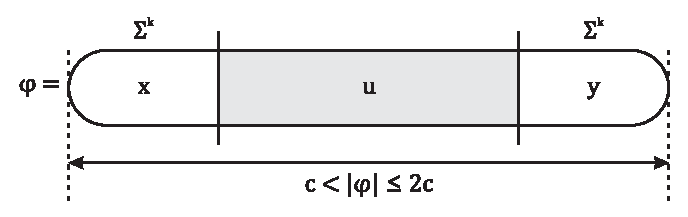
\includegraphics[scale=1.0]{img/instruction_phi.eps}
\caption[The illustration of the instruction $\phi$.]
%$\phi = (x, u \to \Delta^{m_0 + m_2 (i - 1) + j - 1}, y)$.]
{The illustration of the instruction $\phi = (x, u \to \Delta^{m_0 + m_2 (i - 1) + j - 1}, y)$.}
\label{figure:instruction_phi}
\end{figure}

We can easily generalize Lemma \ref{theorem:GsubseteqM} and Lemma \ref{theorem:MsubseteqG} to fit to our case and prove that $L_C(M) = L(G') \cup \{ \lambda \}$. We omit these obvious proofs and verify only that the resulting automaton $M$ has the desired properties. The properties \ref{request:m_0}, \ref{request:m_2} and \ref{request:k} can be easily verified. The only interesting property is the property \ref{request:m_1}. Consider any instruction $(x, u \to \Delta^{m_0 + m_2 (i - 1) + j - 1}, y) \in \Phi_2$, where $i \in \{1, 2, \ldots, m\}$ and $j \in \{1, 2, \ldots, m_2\}$. We know that $|x| = |y| = k$ and $|xuy| > c = U + m_1 - 1$. Therefore, $|u| \ge m_0 + m_1 + m_2 m - 1$. Since $m_0 + m_2 (i - 1) + j - 1 \le m_0 + m_2 m - 1$, we immediately get that $|u| - |\Delta^{m_0 + m_2 (i - 1) + j - 1}| \ge m_1$.

The following lemma will be important later:

\begin{lemma}\label{lemma:dxclra_t}
For each $t \ge 1$, we can set the parameters $m_1$ and $k$ in such a way, that for each instruction $(x, u \to \Delta^r, y) \in \Phi_2$, there exists a subword $v \in \Sigma^*$ (not containing $\Delta$) in the word $u$ with the length $|v| \ge t$. Moreover, $m_1, k = \Theta(t)$. The parameters $m_0$ and $m_2$ can be chosen arbitrarily.
\end{lemma}

\begin{proof}
Set $k := t$ and $m_1 := 2 t + m_2 m - 1$. Consider any instruction $(x, u \to \Delta^r, y) \in \Phi_2$. If $u \in \Sigma^*$ then $v := u$ and we obtain $|v| = |u| > m_1 > t$. Suppose that there are some letters $\Delta$ in $u$. If we can find two consecutive continuous sequences of letters $\Delta$ in $u$, then at least $k$ letters from $\Sigma$ separate these two sequences. We can set $v$ to be this separator. Suppose that there is only one continuous sequence of letters $\Delta$, i.\,e.\ $u = w_1 \Delta^s w_2$ for some $w_1, w_2 \in \Sigma^*$. We know that $|w_1| + s + |w_2| - r \ge m_1$. On the other hand, $|w_1| + s + |w_2| - r \le |w_1| + |w_2| + m_2 m - 1$, since $m_0 \le r, s \le m_0 + m_2 m - 1$. Accordingly, $|w_1| + |w_2| + m_2 m - 1 \ge m_1$. The longer of the words $w_1$, $w_2$ has the length at least $\frac{1}{2}(m_1 - m_2 m + 1) = t$.
\end{proof}

In the following, we outline the basic idea behind the transformation of a $\DXclRA$ $M$ obtained from the previous construction into an equivalent $\DclRA$ $N$. First suppose that we do this transformation in a trivial way, i.\,e.\ we transform each instruction $\phi = (x, u \to \Delta^r, y)$ of $M$, where $r > 1$ and $u = u_1 \ldots u_s$, into the following set of so-called \emph{partial instructions}:
$$
\begin{array}{ll}
\phi_1 & = (x, \underline{u_1} \to \Delta, u_2 u_3 \ldots u_s y),\\
\phi_2 & = (x \Delta, \underline{u_2} \to \Delta, u_3 u_4 \ldots u_s y),\\
\ldots\\
\phi_{r-1} & = (x \Delta^{r-2}, \underline{u_{r-1}} \to
\Delta, u_r u_{r+1} \ldots u_s y),\\
\phi_r & = (x \Delta^{r-1}, \underline{u_r u_{r+1} \ldots u_s} \to \Delta, y).
\end{array}
$$
Apparently, this technique gives us only the inclusion $L(M) \subseteq L(N)$. The other inclusion is not guaranteed. The problem is that we can find two different instructions $\phi$ and $\psi$ in $M$ such that they have different partial instructions $\phi_i$ and $\psi_j$ applicable in the same context. One possible way how to avoid such situations is to introduce some new special instructions, which will encode some extra information into $u$ by rewriting some letters with auxiliary $\Delta$-symbols. By using Lemma \ref{lemma:dxclra_t} we can guarantee a long enough subword $v \in \Sigma^*$ in $u$, which we can use to encode this information. In the rest of this section we describe how to accomplish this task by using one specific coding. Before we jump into the description of the coding, we introduce a useful algorithmic viewpoint, which resembles interactive protocols or even Arthur-Merlin games from the complexity theory. This viewpoint will later simplify many complex constructions used in this section.

\subsection{Algorithmic Viewpoint}\label{section:dxclra_viewpoint}

Let $\Sigma$ be an input alphabet not containing the sentinels $\cent$ and $\$$. Consider two nondeterministic machines: the \emph{querier} $Q$, the \emph{solver} $S$, and the \emph{protocol} \ref{algorithm:dxclra_protocol}.

\begin{algorithm}
\SetKwInOut{Input}{Input}\SetKwInOut{Output}{Output}
\caption{Protocol for the querier $Q$ and the solver $S$.}
\label{algorithm:dxclra_protocol}
\DontPrintSemicolon
\LinesNumbered
\Input{Word $u \in \Sigma^*$.}
\nonl Let $w \leftarrow \cent \cdot u \cdot \$$.\;
\nonl \While{\textbf{true}}{
Ask the querier $Q$ to choose a subword $x$ of $w$, i.\,e.\ $w = w_1 x w_2$.\;
If the solver $S$ accepts $x$ then \textbf{Accept} and \textbf{Halt}.\;
If the solver $S$ answers $y$ on the input $x$ then $w \leftarrow w_1 y w_2$.\;}
\end{algorithm}

The protocol $(Q, S)$ accepts a word $u$ if and only if there exists an accepting computation. Let $L(Q, S)$ denotes the language recognized by the protocol $(Q, S)$:
$$L(Q, S) = \{\ u\ \mid \text{ protocol } (Q, S) \text{ accepts } u\ \}.$$

Consider a class of queriers $\calQ$ and a class of solvers $\calS$. Then $\calL{\calQ, \calS}$ denotes the class of languages recognized by these queriers and solvers:
$$\calL{\calQ, \calS} = \{\ L(Q, S)\ \mid\  Q \in \calQ, S \in \calS\ \}.$$

In the following we will consider only the class of queriers $\calQ = \{Q_1, Q_2, \ldots\}$, such that each querier $Q_K \in \calQ$ for the given input word $w$ chooses nondeterministically an arbitrary subword $x$ of the word $w$ of the length $|x| \le K$.

The only constraint we put on the solver $S$ is that it should preserve the sentinels $\cent$ and $\$$. In other words, the solver can neither erase these sentinels, nor create new ones. We are not interested in the time or space complexity of the solver $S$.

On the other hand, depending on the additional constraints that we put on the solvers we can obtain different classes of solvers, and therefore also different classes of languages $\calL{\calQ, \calS}$. In the following we list several examples.

\begin{enumerate}
\item\label{solver:cl}
Consider the class of solvers $\calS_{cl}$, such that each solver $S \in \calS_{cl}$ works according to the following schema:
\begin{enumerate}
\item \label{solver:c1:a}
      if the input word $x = \cent \cdot \lambda \cdot \$$ then
      \textbf{Accept},
\item \label{solver:c1:b}
      otherwise, either \textbf{Reject}, or return $y$, which can be
      obtained from $x$ by deleting some subword of $x$ (and
      preserving the sentinels $\cent$ a $\$$).
\end{enumerate}
It is easy to see that $\calL{\calQ, \calS_{cl}} = \calL{\clRA}$.

The inclusion $\calL{\clRA} \subseteq \calL{\calQ, \calS_{cl}}$ is trivial. Suppose that $M = (\Sigma, \Phi)$ is a $\clRA$. Let $K = |M|$ be the maximal width of instructions of $M$. The solver $S$ will work according to the above schema in such a way that it will erase a substring from the given input word $x$ only if there exists an instruction of the automaton $M$ which allows such erasing. Apparently, $L(Q_K, S) = L(M)$. For the proof of the other inclusion $\calL{\calQ, \calS_{cl}} \subseteq \calL{\clRA}$ we use the fact the the querier only asks queries with the length bounded above by some constant $K$. Suppose that we have a protocol $(Q_K, S)$, where the solver $S$ works according to the above schema. There exist only finite many different queries the querier $Q_K$ may ask. For each such query $x$ we can describe the behavior of the solver $S$ on the input $x$ by using only the instruction of clearing restarting automata. If we unite all such instructions over all the queries the querier $Q_K$ may ask then we get the required $\clRA$ $M$, such that $L(M) = L(Q_K, S)$.

\item\label{solver:dcl}
The class $\calS_{\Delta cl}$ consists of such solvers $S$ that work according to the same schema as presented in \ref{solver:cl} with the only exception: in the case \ref{solver:c1:b}, the solver $S$ can leave a mark $\Delta \notin \Sigma$ at the place of deleting. Apparently, $\calL{\calQ, \calS_{\Delta cl}} = \calL{\DclRA}$.

\item\label{solver:dxcl}
By analogy, consider the class $\calS_{\Delta^* cl}$ which consists of solvers working according to the schema presented in \ref{solver:cl} with the only exception: in the case \ref{solver:c1:b} the solver $S$ can leave a continuous segment $\Delta^r$ at the place of deleting, where $\Delta \notin \Sigma$ and $r$ is bounded from above by the length of the deleted subword. Not surprisingly, $\calL{\calQ, \calS_{\Delta^* cl}} = \calL{\DXclRA}$.

\item\label{solver:cfl}
The class $\calS_{\textsf{CFL}}$ consists of such solvers $S$ that work according to the following schema:
\begin{enumerate}
\item \label{solver:cfl:a}
      if $x = \cent \cdot N_1 \cdot \$$ then \textbf{Accept},
\item \label{solver:cfl:b}
      if $x$ contains $\cent$ or $\$$ then \textbf{Reject},
\item \label{solver:cfl:c}
      if $x$ contains neither $\cent$, nor $\$$, then either
      \textbf{Reject}, or return a nonterminal.
\end{enumerate}
We prove that $\calL{\calQ, \calS_{\textsf{CFL}}} = \CFL$.

$\CFL \subseteq \calL{\calQ, \calS_{\textsf{CFL}}}$: Let $G = (V_N, V_T, N_1, P)$ be a context-free grammar with $V_N = \{N_1, \ldots, N_m\}$, and $\cent, \$ \notin V_N \cup V_T$. Let $K$ be the length of the longest right-hand side of productions from $P$. The corresponding solver $S$ will work according to the above schema in such a way, that in the case \ref{solver:cfl:c} $S$ returns the nonterminal $N_i$ only if $(N_i \to x) \in P$. Apparently, $L(Q_K, S) = L(G)$.

$\calL{\calQ, \calS_{\textsf{CFL}}} \subseteq \CFL$: There exist only finite many different queries the querier $Q_K$ may ask. For each such query $x$ we can describe the behavior of the solver $S$ on the input $x$ by using context-free productions of the form $(N_i \to x)$. If we unite all such productions over all the queries the querier $Q_K$ may ask then we get the required context-free grammar $G$, such that $L(G) = L(Q_K, S)$.

\item\label{solver:csl}
The class $\calS_{\textsf{CSL}}$ consists of such solvers $S$ that work according to the same schema as presented in \ref{solver:cfl} with the only exception: in the case \ref{solver:cfl:c}, the solver $S$ can rewrite any subword of the input word $x$ to a nonterminal $N_i$. Analogously, $\calL{\calQ, \calS_{\textsf{CSL}}} = \CSL$.
\end{enumerate}

In this way we can characterize also other language classes, such as pure languages \cite{maurer1980pure} etc. However, the most important contribution of these protocols is that we no longer perceive $\clRA$ ($\DclRA$, $\DXclRA$, respectively) as a mere set of instructions, but rather as a nondeterministic machine $S$ with an unbounded computational power working according to a particular schema. Instead of giving a list of instructions we rather describe the algorithm behind the corresponding solver. Now consider a $\DXclRA$ whose construction was based on a given context-free grammar $G$. Our goal is to construct a solver $S \in \calS_{\Delta cl}$, which will be able to imitate the work of the automaton $M$ by splitting every instruction of $M$ into several steps. In the first phase, the solver $S$ will encode (by using a special coding) some information into the tape specifying which instruction of $M$ it is going to execute. In the second phase, the solver $S$ will actually execute the chosen instruction (step by step). The coding will be designed in such a way that it will be possible to unambiguously interpret the content of the input tape at any given time.

\subsection{Coding}\label{section:dxclra_coding}

Consider a finite nonempty alphabet $\Sigma$ and $\Delta \notin \Sigma$. Our goal is to describe a mechanism which would enable us to encode any information to an arbitrary, sufficiently long word $w \in \Sigma^*$, only by replacing some letters of $w$ by symbols $\Delta$. Moreover, we require that it should be possible to recover the original word $w$ at any time.

\begin{theorem}[Coding 1]\label{theorem:dxclra_coding_1}
Let $\Sigma$ be a finite nonempty alphabet and $\Delta \notin \Sigma$. Then there exist a positive integer $B$ and a table $T$ of triples $(x, z, y)$, $xzy \in \Sigma^B$, $z \in \Sigma$, such that:
\begin{enumerate}
\item\label{theorem:dxclra_coding_1:a} $\{ xzy \mid (x, z, y) \in T \} = \Sigma^B$,
\item\label{theorem:dxclra_coding_1:b} For every $(x, y)$, $xy \in \Sigma^{B-1}$ there exists exactly one $z \in \Sigma: (x, z, y) \in T$.
\end{enumerate}
\end{theorem}

This theorem guarantees that if we take any word $w \in \Sigma^B$ then there exists a factorization $w = xzy$, such that $(x, z, y) \in T$. Now if we replace the letter $z$ by $\Delta$, we do not lose any information, since we are able to recover the letter $z$ from the context $(x, y)$ by using the table $T$.

\begin{proof}
Let us set $B = |\Sigma|$ and define a bipartite graph $G = (U \cup V, E)$ as follows:
\begin{enumerate}
\item $U = \Sigma^B$,
\item $V = (\Sigma \cup \{\Delta\})^B \cap (\Sigma^* \cdot \Delta \cdot \Sigma^*)$,
\item $E = \{ \{u, v\} \mid u \in U, v \in V, u = xzy, v = x \Delta y\}$.
\end{enumerate}
There is an edge $\{u, v\} \in E$ between $u \in U$ and $v \in V$ if and only if $v$ can be obtained from $u$ by replacing one of its letters by the symbol $\Delta$ (see Figure \ref{figure:graph}).
\begin{figure}[htp]
\centering
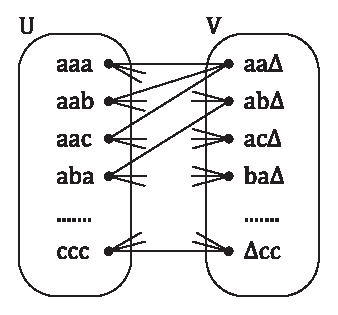
\includegraphics[scale=1.0]{img/graph.eps}
\caption[Bipartite graph $G = (U \cup V, E)$ for $\Sigma = \{a, b, c\}$.]
{Bipartite graph $G = (U \cup V, E)$ for $\Sigma = \{a, b, c\}$.}
\label{figure:graph}
\end{figure}
It is easy to see, that:
\begin{enumerate}
\item $|U| = |\Sigma^B| = B^B$,
\item $|V| = B |\Sigma|^{B-1} = B^B$.
\end{enumerate}
Moreover, the degree of each $u \in U$ in $G$ is $B = |\Sigma|$ and the degree of each $v \in V$ in $G$ is $|\Sigma|$. Therefore, $G$ is a $|\Sigma|$-regular bipartite graph. According to Hall's Theorem \cite{Hall1935} there exists a perfect matching in $G$, which gives us the required table $T$.
\end{proof}

\begin{example}\label{example:dxclra_ab}
Consider $\Sigma = \{a, b\}$. The adjacency matrix of the corresponding bipartite graph $G$ used in the proof of Coding 1 Theorem \ref{theorem:dxclra_coding_1} is shown in Table \ref{table:dxclra_example:dxclra_ab}.
\begin{table}[ht]
\centering
\begin{tabular}{| c || c | c | c | c |}
 \hline
     &  $a \Delta$  &   $b \Delta$&  $\Delta a$  &  $\Delta b$  \\
\hline\hline
$aa$ & $\mathbf{\underline{1}}$ &      $0$     &      $1$     &    $0$\\
\hline
$ab$ &      $1$     &      $0$     &      $0$     & $\mathbf{\underline{1}}$\\
\hline
$ba$ &      $0$     &      $1$     & $\mathbf{\underline{1}}$ &    $0$\\
\hline
$bb$ &      $0$     & $\mathbf{\underline{1}}$ &      $0$     &    $1$\\
\hline
\end{tabular}
\caption{Adjacency matrix for $\Sigma = \{a, b\}$.}
\label{table:dxclra_example:dxclra_ab}
\end{table}
The highlighted perfect matching gives us the following bijection:
$$aa \leftrightarrow a \Delta,
\ \ ab \leftrightarrow \Delta b,
\ \ ba \leftrightarrow \Delta a,
\ \ bb \leftrightarrow b \Delta,$$
and the corresponding table $T = \{
\ (a, a, \lambda),
\ (\lambda, a, b),
\ (\lambda, b, a),
\ (b, b, \lambda)\ \}$.
\end{example}
\begin{example}\label{example:dxclra_abc}
For $\Sigma = \{a, b, c\}$ we only give the resulting bijection:
\begin{center}
\begin{tabular}{lllll}
  $aaa \leftrightarrow \Delta a a$,\quad\quad
& $aab \leftrightarrow \Delta a b$,\quad\quad
& $aac \leftrightarrow a a \Delta$,\quad\quad
& $aba \leftrightarrow \Delta b a$,\quad\quad
& $abb \leftrightarrow a \Delta b$,\\
  $abc \leftrightarrow a b \Delta$,
& $aca \leftrightarrow a \Delta a$,
& $acb \leftrightarrow a c \Delta$,
& $acc \leftrightarrow a \Delta c$,
& $baa \leftrightarrow b \Delta a$,\\
  $bab \leftrightarrow b \Delta b$,
& $bac \leftrightarrow b a \Delta$,
& $bba \leftrightarrow b b \Delta$,
& $bbb \leftrightarrow \Delta b b$,
& $bbc \leftrightarrow \Delta b c$,\\
  $bca \leftrightarrow \Delta c a$,
& $bcb \leftrightarrow b c \Delta$,
& $bcc \leftrightarrow b \Delta c$,
& $caa \leftrightarrow c \Delta a$,
& $cab \leftrightarrow c a \Delta$,\\
  $cac \leftrightarrow \Delta a c$,
& $cba \leftrightarrow c b \Delta$,
& $cbb \leftrightarrow c \Delta b$,
& $cbc \leftrightarrow c \Delta c$,
& $cca \leftrightarrow c c \Delta$,\\
  $ccb \leftrightarrow \Delta c b$,
& $ccc \leftrightarrow \Delta c c$.
\end{tabular}
\end{center}

Next consider the following sample word:
$$w = acc bab cca caa bbc abc bca caa.$$
Let us factorize this word $w$ into the groups consisting of $B = 3$ letters:
$$w\ =\ acc\ \mid\ bab\ \mid\ cca\ \mid\ caa\ \mid\ bbc\ \mid\ abc\ \mid\ bca\ \mid\ caa.$$
Suppose that we want to encode the information $i = 11001010$ into the word $w$ without losing any information. We can achieve this by \emph{marking} the groups of $w$ by $\Delta$ that correspond to $1$s in the information $i$. If we use the above bijection we will be able to recover the original word $w$. After encoding the information $i$ we get the following word:
$$w'\ =\ a \Delta c\ \mid\ b \Delta b\ \mid\ c c a\ \mid\ c a a\ \mid
       \ \Delta b c\ \mid\ a b c\ \mid\ \Delta c a\ \mid\ c a a.$$
\end{example}

By applying the encoding from Example \ref{example:dxclra_abc} we can store an $n$-bit information in any word $w$ of length at least $n B$. However, we need to ``see'' the whole word $w$ in order to correctly define the groups of $B$ letters.

The perfect matching of a regular bipartite graph $G$ can be found effectively with respect to the size of the graph $G$. However, the table defining the bijection contains $|\Sigma|^{|\Sigma|}$ entries.  The question is, whether we can compute the bijection in polynomial time w.r.t. $|\Sigma|$ without precomputing the whole table $T$? The answer is yes. Let us assign to every $a \in \Sigma$ some value $\nu(a) \in \{1, \ldots, |\Sigma|\}$ bijectively, and define $\nu^*(w_1 \ldots w_n) = \sum_{i = 1}^{n} \nu(w_i) \mod |\Sigma|$, for all $w_1 \ldots w_n \in \Sigma^*$. The table $T$ consists of all triples of the form $(x, z, y)$, where $x, y \in \Sigma^*$, $z \in \Sigma$, $|xzy| = |\Sigma|$, and $\nu^*(xzy) = |x|$. Given any $w \in \Sigma^{|\Sigma|}$ we can effectively factorize $w$ to $xzy$, such that $(x, z, y) \in T$, by defining $|x| = \nu^*(w)$. This proves that $\{ xzy \mid (x, z, y) \in T \} = \Sigma^{|\Sigma|}$. Since $z$ is uniquely determined by the contexts $(x, y)$, $T$ satisfies both conditions \ref{theorem:dxclra_coding_1:a}, \ref{theorem:dxclra_coding_1:b} of Theorem \ref{theorem:dxclra_coding_1}, and we do not need to store it explicitly.

As we can see, the coding introduced in Coding 1 Theorem \ref{theorem:dxclra_coding_1} is \emph{length-preserving}. It means, that if we encode an information into a word $w$, the length of the word remains preserved. The question is, whether we can find a \emph{length-reducing} coding. The answer is: yes, trivially. Consider the following word:
$$w = ababaababbbaabaa.$$
First, we group together consecutive letters of $w$:
$$w = \underline{ab}\ \underline{ab}\ \underline{aa}
\ \underline{ba}\ \underline{bb}\ \underline{ba}
\ \underline{ab}\ \underline{aa}.$$
Now consider the word $w$ as a word over the \emph{pair} alphabet:
$$\underline{\Sigma} = \{\underline{aa}, \underline{ab},
\underline{ba}, \underline{bb}\}.$$
If we apply the length-preserving coding of Coding 1 Theorem \ref{theorem:dxclra_coding_1} on the pair alphabet $\underline{\Sigma}$, we automatically get a length-reducing coding over the original alphabet $\Sigma$. This is because the rewriting of one letter from the pair alphabet $\underline{\Sigma}$ by $\Delta$ is equivalent to the rewriting of two letters from the original alphabet $\Sigma$ by $\Delta$. However, in this case $B = 2|\underline{\Sigma}| = 2|\Sigma|^2$. For example, for $\Sigma = \{a, b\}$ we need groups of $B = 2|\Sigma|^2 = 8$ letters. Can we do better? The answer is: yes, but not too much.

\begin{theorem}[$\kappa$-Reducing Coding 1]
\label{theorem:dxclra_k_reducing_coding_1}
Let $\kappa$ be a nonnegative integer, $\Sigma$ a finite nonempty alphabet and $\Delta \notin \Sigma$. Then there exist a positive integer $B$ and a table $T$ of triples $(x, z, y)$, $xzy \in \Sigma^B$, $z \in \Sigma^{\kappa+1}$, such that:
\begin{enumerate}
\item\label{theorem:dxclra_k_reducing_coding_1:a} $\{ xzy \mid (x, z, y) \in T \} = \Sigma^B$,
\item\label{theorem:dxclra_k_reducing_coding_1:b} For every $(x, y)$, $xy \in \Sigma^{B-\kappa-1}$ there exists exactly one $z \in \Sigma^{\kappa+1}$ such that $(x, z, y) \in T$.
\end{enumerate}
\end{theorem}

\begin{proof}
Again, consider a bipartite graph $G = (U \cup V, E)$, where:
\begin{enumerate}
\item $U = \Sigma^B$,
\item $V = (\Sigma \cup \{\Delta\})^{B-\kappa} \cap (\Sigma^* \cdot \Delta \cdot \Sigma^*)$,
\item $E = \{ \{u, v\} \mid u \in U, v \in V, u = xzy, v = x \Delta y\}$.
\end{enumerate}
There is an edge $\{u, v\} \in E$ between $u \in U$ and $v \in V$ if and only if $v$ can be obtained from $u$ by replacing one of its subwords $z \in \Sigma^{\kappa+1}$ by $\Delta$. If we define $B = |\Sigma|^{\kappa+1} + \kappa$ then we get the equality $|U| = |V|$, because:
\begin{enumerate}
\item $|U| = |\Sigma^B| = |\Sigma|^B$,
\item $|V| = (B - \kappa) |\Sigma|^{B - \kappa - 1} = |\Sigma|^{\kappa+1} |\Sigma|^{B - \kappa - 1} = |\Sigma|^B$.
\end{enumerate}
Moreover, the degree of each $u \in U$ in $G$ is $B - \kappa = |\Sigma|^{\kappa+1}$ and the degree of each $v \in V$ in $G$ is $|\Sigma|^{\kappa+1}$. Therefore, $G$ is a $|\Sigma|^{\kappa+1}$-regular bipartite graph. According to Hall's Theorem \cite{Hall1935} there exists a perfect matching in $G$, which gives us the required table $T$.
\end{proof}

For example, for $\Sigma = \{a, b\}$ the $1$-Reducing Coding 1 gives us $B = |\Sigma|^{\kappa+1} + \kappa = 5$, which is an improvement to $B = 8$.

The obvious problem with Coding 1 is that we need to ``see'' the whole word $w$ in order to correctly define the groups of $B$ letters. One possible way how to avoid this problem is to find a coding that is not dependent on any specific factorization of the word to the groups of letters. Our goal is to recover the original letters hidden by the symbols $\Delta$ only with the knowledge of local contexts of these symbols $\Delta$.

\begin{theorem}[Coding 2]\label{theorem:dxclra_coding_2}
Let $\Sigma$ be a finite nonempty alphabet and $\Delta \notin \Sigma$. Then there exist positive integers $B$, $K$, and a table $T$ of triples $(x, z, y)$, $x, y \in \Sigma^K$, $z \in \Sigma$, such that:
\begin{enumerate}
\item\label{theorem:dxclra_coding_2:a}
For every context $(x, y) \in \Sigma^K \times \Sigma^K$ there exists at most one $(x, z, y) \in T$.
\item\label{theorem:dxclra_coding_2:b} For every word $w \in \Sigma^B$ there exists at least one $(x, z, y) \in T$ such that $xzy$ is a subword of $w$.
\end{enumerate}
\end{theorem}

Apparently, we can replace the letter $z$ by $\Delta$ in the subword $xzy$ of $w$ without losing any information, because we can recover $z$ from the context $(x, y)$.

\begin{proof}
(Induction by $|\Sigma|$). For $\Sigma = \{a, b\}$ let us set $B = 8$, $K = 2$, and
\begin{center}
\begin{tabular}{c c c c c c}
$T = \{$ &
   $(aa, a, aa)$,& $(ab, a, aa)$,& $(ba, b, aa)$,& $(bb, a, aa)$,& \\
 & $(aa, a, ab)$,& $(ab, a, ab)$,& $(ba, b, ab)$,& $(bb, a, ab)$,& \\
 & $(aa, b, ba)$,& $(ab, a, ba)$,& $(ba, b, ba)$,& $(bb, b, ba)$,& \\
 & $(aa, b, bb)$,& $(ab, a, bb)$,& $(ba, b, bb)$,& $(bb, b, bb)$ & $\}\;.$\\
\end{tabular}
\end{center}
The condition \ref{theorem:dxclra_coding_2:a} obviously holds. The condition
\ref{theorem:dxclra_coding_2:b} is verified in Table \ref{table:dxclra_verify2}.

\begin{table}[ht]
\centering
\begin{tabular}{c c c c}
\hline \hline
\underline{aaaaa}??? & \underline{aaaab}??? &
aa\underline{abaaa}? & aa\underline{abaab}?\\
aa\underline{ababa}? & aa\underline{ababb}? &
a\underline{aabba}?? & a\underline{aabbb}??\\
a\underline{abaaa}?? & a\underline{abaab}?? &
a\underline{ababa}?? & a\underline{ababb}??\\
\underline{aabba}??? & \underline{aabbb}??? &
\underline{abaaa}??? & \underline{abaab}???\\
\underline{ababa}??? & \underline{ababb}??? &
a\underline{bbaaa}?? & a\underline{bbaab}??\\
ab\underline{babaa}? & ab\underline{babab}? &
ab\underline{babba}? & ab\underline{babbb}?\\
ab\underline{bbaaa}? & ab\underline{bbaab}? &
abb\underline{babaa} & abb\underline{babab}\\
abb\underline{babba} & abb\underline{babbb} &
a\underline{bbbba}?? & a\underline{bbbbb}??\\
b\underline{aaaaa}?? & b\underline{aaaab}?? &
baa\underline{abaaa} & baa\underline{abaab}\\
baa\underline{ababa} & baa\underline{ababb} &
ba\underline{aabba}? & ba\underline{aabbb}?\\
ba\underline{abaaa}? & ba\underline{abaab}? &
ba\underline{ababa}? & ba\underline{ababb}?\\
b\underline{aabba}?? & b\underline{aabbb}?? &
\underline{babaa}??? & \underline{babab}???\\
\underline{babba}??? & \underline{babbb}??? &
\underline{bbaaa}??? & \underline{bbaab}???\\
b\underline{babaa}?? & b\underline{babab}?? &
b\underline{babba}?? & b\underline{babbb}??\\
b\underline{bbaaa}?? & b\underline{bbaab}?? &
bb\underline{babaa}? & bb\underline{babab}?\\
bb\underline{babba}? & bb\underline{babbb}? &
\underline{bbbba}??? & \underline{bbbbb}???\\
\hline
\end{tabular}
\caption{All possibilities for $w \in \Sigma^K$.}
\label{table:dxclra_verify2}
\end{table}

Note that $T$ can be shortly described as $T = \{ (xx, y, y?) \mid x, y \in \Sigma \} \cup \{ (xy, x, ??) \mid x \neq y; x, y \in \Sigma \}$,  where the symbol $?$ is a placeholder for an arbitrary letter from $\Sigma$. We can avoid using the symbol $?$ completely by writing $T = \{ (xx, y, y) \mid x, y \in \Sigma \} \cup \{ (xy, x, \lambda) \mid x \neq y; x, y \in \Sigma \}$. In other words, we allow using triples $(l, z, r)$, where $|l| < K$ or $|r| < K$ (or both). This is not a problem since we can easily extend the left context (right context, respectively) to be from $\Sigma^K$ by adding (all possible combinations of) ``dummy'' letters from $\Sigma$ to the left of the left context $l$ (to the right of the right context $r$, respectively). The reason why $T$ satisfies the condition \ref{theorem:dxclra_coding_2:b} is as follows. Consider a sufficiently long word $w \in \Sigma^*$. There are only two cases: either each (internal) letter in $w$ is doubled, i.\,e.\ each (internal) letter $x$ in $w$ has a neighbor $x$, or there exists an (internal) letter $x$ in $w$ which does not have a neighbor $x$. In the first case the pattern $xxyy$ will occur, and in the second case the pattern $xyx$, where $x \neq y$, will occur.

The proof of the induction step was provided by a Russian mathematician Ilya Bogdanov on the following website: \url{http://mathoverflow.net/questions/76326/can-you-hide-a-letter-without-losing-information}. Let us assume that we know the positive integers $B'$, $K'$, and the table $T'$ of triples for some alphabet $\Sigma'$. Our goal is to find the positive integers $B$, $K$, and the table $T$ of triples (satisfying both conditions  \ref{theorem:dxclra_coding_2:a}, \ref{theorem:dxclra_coding_2:b}) for the extended alphabet $\Sigma = \Sigma' \cup \{x\}$, where $x \notin \Sigma'$. Let us assume that $K' \ge 2|\Sigma'|$. We claim that we can set $K = B'$. For convenience, we say that we \emph{catch} the word $w \in \Sigma^*$ if there exists at least one $(x, z, y) \in T$ such that $xzy$ is a subword of $w$ (i.\,e.\ the condition \ref{theorem:dxclra_coding_2:b} holds for the word $w$). Our goal is to catch all long enough words (i.\,e.\ all words from $\Sigma^B$ for some positive integer $B$). First, let us reuse all triples from $T'$, except that we need to prolong their contexts to the length $K$. By using the triples from $T'$ we can catch every word $w \in \Sigma^*$ that contains a subword $w'$ over $\Sigma'$ of  length at least $B'$ (where this subword stands at least $K$ letters from the beginning of the word $w$ to leave enough room for the prolonged contexts). Second, we need to catch also all other words. These words contain subwords of the form $xw'x$, where $0 \le |w'| < B'$ and $w'$ does not contain $x$ (again we consider only subwords $xw'x$ standing at least $K$ letters from the beginning). Let $xw'x$ be any such subword with the maximal possible length. We distinguish three cases: (1) $|w'|$ is at least $2 |\Sigma'|$, (2) $|w'|$ is at least $|\Sigma'|$, but less than  $2 |\Sigma'|$, and (3) $|w'|$ is less then $|\Sigma'|$.
\begin{enumerate}
\item[(1)] In case $|w'| \ge 2 |\Sigma'|$ we can reuse the idea of Coding 1 (see Theorem \ref{theorem:dxclra_coding_1}). Let us assign to every $a \in \Sigma'$ some value $\nu(a) \in \{1, \ldots, |\Sigma'|\}$ bijectively, and define $\nu^*(w_1 \ldots w_n) = \sum_{i = 1}^{n} \nu(w_i) \mod |\Sigma'|$. Let us add to $T$ all triples of the form $(xu, a, vx)$, where $u, v$ are words over $\Sigma'$, $a \in \Sigma'$, $0 \le |u| < |\Sigma'|$, $|\Sigma'| \le |v| < B'$, $2|\Sigma'| \le |uav| < B'$, and $\nu^*(uav) = |u|$. Now if we have any subword $xw'x$ with $|w'| \ge 2 |\Sigma'|$, then we set $u$ to be the prefix of $w'$ of length $\nu^*(w')$, $a$ to be the next letter of $w'$, and $v$ to be the remaining suffix of $w'$. It is easy to see that $\nu^*(uav) = \nu^*(w') = |u|$, i.\,e.\ our word $w$ is caught by a triple $(xu, a, vx) \in T$. Since $a$ is determined uniquely by $u$ and $v$, these triples satisfy the condition \ref{theorem:dxclra_coding_2:a}.
\item[(2)] In case $|\Sigma'| \le |w'| < 2 |\Sigma'|$ we use the triples of the form $(xu, x, \lambda)$, where $u$ is over $\Sigma'$ and $|\Sigma'| \le |u| < 2 |\Sigma'|$. Note that these triples do not interfere with the triples from (1), because here $|\Sigma'| \le |u|$.
\item[(3)] Finally, if $|w'| < |\Sigma'|$ we use the triples of the form $(xu, x, vx)$, where $u, v$ are words over $\Sigma'$, and $0 \le |u|, |v| < |\Sigma'|$. These triples do not interfere with the triples from (1), because here we have $|v| < |\Sigma'|$. They do not interfere with the triples from (2), because here we have $|u| < |\Sigma'|$.
\end{enumerate}
To formally prove the condition \ref{theorem:dxclra_coding_2:a}, let $(l, r) \in \Sigma^K \times \Sigma^K$. If $\Suff_{2|\Sigma'|}(l)$ does not contain $x$, then only a triple from $T'$ can match the context $(l, r)$. This is because all triples from $T'$ have contexts of length $K' \ge 2|\Sigma'|$, and all other triples from $T$ contain $x$ in $\Suff_{2|\Sigma'|}(l)$. In (1) $\Suff_{|\Sigma'|}(l)$ contains $x$, while $\Pref_{|\Sigma'|}(r)$ does not. In (2) $\Suff_{2|\Sigma'|}(l)$ contains $x$, while $\Suff_{|\Sigma'|}(l)$ does not. Finally, in (3) both $\Suff_{|\Sigma'|}(l)$ and $\Pref_{|\Sigma'|}(r)$ contain $x$. It is easy to see that the condition \ref{theorem:dxclra_coding_2:b} is satisfied for long enough words. Let $B = 3B'$ and $w \in \Sigma^B$. If $w$ contains a subword $w'$ over $\Sigma'$ of length at least $B'$ standing at least $K = B'$ letters from the beginning, then it is caught by $T'$. Otherwise, it contains at least two consecutive subwords of the form $xw'x$ standing at least $K$ letters from the beginning, in which case one of the cases (1), (2), (3) applies.
\end{proof}

We will not use Coding 2 in our proof, because Coding 1 is more compact and much simpler. However, as we have already mentioned before, the problem with Coding 1 is that the solver $S \in \calS_{\Delta cl}$ may not be able to decode $\Delta$ symbols in the input word $w$, since $w$ can often be only a small part of the original input tape. If the word $w$ does not start with the left sentinel $\cent$ then we are not able to correctly factorize $w$ into the groups of $B$ letters, and thus we are not able to interpret $\Delta$ symbols occurring in the word $w$.

Fortunately, there exists a simple trick how to avoid this problem. In order to correctly factorize the input word $w$ into groups of $B$ letters we only need some kind of ``fixed point'', which exactly defines the starting position of the first group of the correct factorization. The left sentinel $\cent$ is one example of such fixed point. Thus in the first phase we distribute such fixed points throughout the whole input tape starting at the left sentinel $\cent$. The distances between two consecutive fixed points will be approximately constant. We illustrate this idea on the following simplified example. Suppose that we have the following word:
$$w = abacc \Delta bac bba cac bcb aac bcb acb aca bab$$
The symbol $\Delta$ in $w$ represents our fixed point and defines the following factorization:
$$w = abacc \mathbf{\Delta}\ \mid\ bac\ \mid\ bba\ \mid\ cac\ \mid\ bcb
\ \mid\ aac\ \mid\ bcb\ \mid\ acb\ \mid\ aca\ \mid\ bab$$
We place the next fixed point into the $9$th group to the right from the highlighted fixed point $\mathbf{\Delta}$ (by using the bijection from Example \ref{example:dxclra_abc}):
$$w' = abacc \Delta\ \mid\ bac\ \mid\ bba\ \mid\ cac\ \mid\ bcb\ \mid\ aac\ \mid\ bcb\ \mid\ acb\ \mid\ aca\ \mid\ b \Delta b$$
As you can see, the number of letters between two consecutive fixed points is either  $3 \times 8$, or $3 \times 8 + 1$, or $3 \times 8 + 2$. We place another fixed point whenever the input word $w$ is of the form $w \in \cent \cdot \Sigma^{\ge 3 \times 9}$ or $w \in \Sigma^* \cdot \Delta \cdot \Sigma^{\ge 3 \times 9}$.

\subsection{Idea of the Algorithm}\label{section:dxclra_algorithm}

In this section we describe the algorithm behind the solver $S \in \calS_{\Delta cl}$, which imitates the work of the $\DXclRA$ $M$ constructed according to a given context-free grammar in Chomsky normal form. The automaton $M$ works in a bottom-up fashion. If the automaton recognizes that some subword $w$ of the input tape can be derived from a nonterminal $N_i$, then it can replace the inner part of this subword $w$ by the code $\Delta^r$, where $r = m_0 + m_2 (i - 1) + j - 1$ for some $j \in \{1, 2, \ldots, m_2\}$, leaving the first $k$ letters and the last $k$ letters of $w$ as separators. The segment $\Delta^r$ together with its separators represents a code for the nonterminal $N_i$. These separators have a nice and useful property: if one changes some letters in these separators, the acceptance of the whole word on the input tape remains
unchanged.

Our solver $S$ is not obliged to preserve the representation used by the automaton $M$. Moreover, because of some technical reasons, we will not represent the nonterminal $N_i$ by using a continuous segment $\Delta^r$. Instead, we will use the segment $\Delta x \Delta^{r-4} y \Delta$, where $x, y \in \Sigma$ are the so-called ``holes''. These holes are useful in the sense that they can unambiguously identify the start and the end of the segment $\Delta x \Delta^{r-4} y \Delta$ inside any word marked by other symbols $\Delta$. For example, in the following word:
$$a \Delta c ca\Delta \underline{\Delta b \Delta^{r-4} a \Delta} aab$$
we have underlined such segment with holes. It will be clear later why we need this representation. For convenience, we will often use the following convention: whenever we talk about a \emph{continuous segment $\Delta^r$ with holes}, we will always mean the segment $\Delta x \Delta^{r-4} y \Delta$, where $x, y \in \Sigma$ represent the holes.

In the following we introduce another conventions which will be used later in the description of the resulting algorithm. As we have already explained, if we want to encode the information into some word $w \in \Sigma^*$, we need to know the factorization of this word $w$ into groups of $B$ letters (see Section \ref{section:dxclra_coding}). This factorization (once defined) cannot be changed during the course of the algorithm. Otherwise, we could misinterpret the symbols $\Delta$ occurring in the word $w$. In order to correctly factorize the input word we need to find the so-called \emph{fixed point}. We recognize three types of fixed points:

\begin{enumerate}
\item \emph{Fixed point $\cent$}: In the word $\cent \cdot w$, where $w \in \Gamma^*$, the fixed point $\cent$ defines the following groups:
$$\cent \mid w_1 \mid w_2 \mid w_3 \mid \ldots,$$
where $w = w_1 w_2 w_3 \ldots$, and $|w_1| = |w_2| = |w_3| = \ldots = B$. In other words, the start of the input tape is a fixed point.

\item \emph{Fixed point $\Delta^r$ with holes}: In the word $u w$, where $u$ is the segment $\Delta^r$ with holes, $r = m_0 + m_2 (i - 1) + j - 1$ for some $j \in \{1, 2, \ldots, m_2\}$, the fixed point $u$ defines the following groups:
$$w_0 \mid w_1 \mid w_2 \mid w_3 \mid \ldots,$$
where $u w = w_0 w_1 w_2 \ldots$, $|w_0| = m_0 + m_2 (i - 1)$, and $|w_1| = |w_2| = |w_3| = \ldots = B$. In other words, the segment $\Delta^r$ with holes is a fixed point. Note that $|w_0| \le r$. The reason why we factorize the word $u w$ in this way will be explained later.

\item \emph{Fixed point $\mathbf{u} \Delta \mathbf{v} \Delta$}: In the word $u \Delta v \Delta w$, where $u \in \Sigma^{2B}$, $v \in \Sigma^{\le 2B - 2}$, $w \in \Sigma \cdot \Gamma^*$, the fixed point $\mathbf{u} \Delta \mathbf{v} \Delta$ defines the following groups:
$$u \Delta v \Delta \mid w_1 \mid w_2 \mid w_3 \mid \ldots,$$
where $w = w_1 w_2 w_3 \ldots$, and $|w_1| = |w_2| = |w_3| = \ldots = B$. In other words, two symbols $\Delta$, which are close to each other, represent a fixed point.
\end{enumerate}

To prevent the accidental creation of fixed points of the type $\mathbf{u} \Delta \mathbf{v} \Delta$ we introduce the following convention. We do not encode the information straight into the groups of length $B$, but rather to the so-called \emph{units}. A unit is defined as three consecutive groups of length $B$. If we want to mark a unit in order to encode one bit of information we always mark the middle group of the unit. The first and the third group of the unit serves as separators. Thanks to these separators any two consecutive symbols $\Delta$ in any two neighboring units are separated by at least $2B$ letters from $\Sigma$. We illustrate this idea on the following example. Consider $\Sigma = \{a, b, c\}$ and the following word:
$$abc \Delta^r acc bab cca caa bbc abc bcc caa,$$
where $r = m_0 + m_2 (i - 1)$. The fixed point $\Delta^r$ (with holes) defines the following groups:
$$abc \Delta^r \mid \mid acc \mid \mathbf{bab} \mid cca \mid \mid caa \mid \mathbf{bbc} \mid abc \mid \mid bcc \mid caa,$$
where the units are separated by two lines ($\mid \mid$). The middle groups of the units are in bold.

Note that if we mark two consecutive units, we never get the fixed point of the type $\mathbf{u} \Delta \mathbf{v} \Delta$. However, we can always obtain such a fixed point by marking two consecutive groups, provided that there are at least two unmarked groups preceding the first marked group. We use this observation in the first phase of the algorithm, in which we distribute the fixed points of this type throughout the whole input tape.

In the following we introduce the term \emph{working area}. Consider an input tape with all its fixed points. If we erase these fixed points, the input tape will break into the segments, which we refer to as the working areas (see Figure \ref{figure:tape}).

\begin{figure}[htp]
\centering
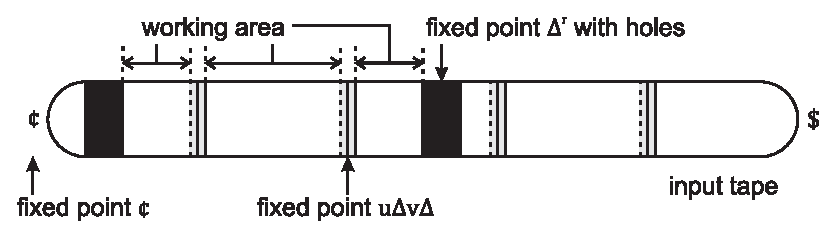
\includegraphics[scale=1.0]{img/tape.eps}
\caption[The segmentation of the input tape into the working areas.]
{The segmentation of the input tape into the working areas.}
\label{figure:tape}
\end{figure}

Fixed points exactly define the factorization into the groups of length $B$ and thus they also define the corresponding units inside these working areas. The term \emph{working space} refers to the longest possible subword of the working area containing only the whole units that can be used to encode some information (see Figure \ref{figure:working_space}).

\begin{figure}[htp]
\centering
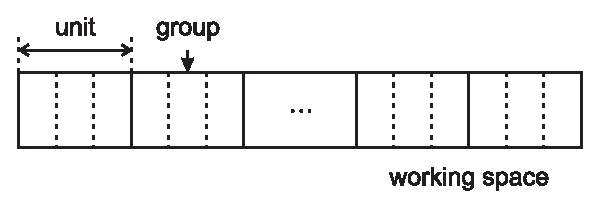
\includegraphics[scale=1.0]{img/working_space.eps}
\caption[Working space divided into the units.]
{Working space divided into the units.}
\label{figure:working_space}
\end{figure}

Since we encode the information only into the middle groups of the units, no fixed points can be created in this way. However, there is one special exception. During the computation the algorithm gets into a state in which it starts to create a new continuous segment $\Delta^r$ (with holes) somewhere inside the working space. This segment will (after completing) represent a code for a nonterminal. By definition, the completed segment $\Delta^r$ (with holes) represents also a new fixed point. This could be a problem, since the process of the execution of the instruction of the automaton $M$ is not yet completed at this stage. In order to finish this process we must also clear the remaining letters on both sides of the newly created segment $\Delta^r$ (with holes). The problem is, that a new fixed point could break the correctness of the previously defined factorization into the groups of length $B$. Therefore, in the following we introduce some new terms that will enable us to solve this problem.

The working area is called \emph{empty} if it does not contain a subword $u \Delta v$, where $u, v \in \Sigma^{4L}$. Otherwise we call the working area \emph{reserved}. Next, we will distinguish between \emph{valid} and \emph{invalid} fixed points. The fixed points of the types $\cent$ and $\mathbf{u} \Delta \mathbf{v} \Delta$ are always valid. The fixed point of the type $\Delta^r$ (with holes) is valid only if there exists at least one empty working area adjacent to this fixed point. Otherwise, the fixed point $\Delta^r$ (with holes) is invalid. Thus, if we want to make the fixed point $\Delta^r$ (with holes) invalid, we only need to place this fixed point between two marked units.

Now we are ready to give the details of the algorithm imitating the work of the $\DXclRA$ $M$ (see Algorithm \ref{algorithm:dxclra_solver}).

\begin{algorithm}
\SetKwInOut{Input}{Input}\SetKwInOut{Output}{Output}
\caption{Algorithm behind the solver $S \in \calS_{\Delta cl}$ imitating the work of the $\DXclRA$ $M = (\Sigma, \Phi)$.}
\label{algorithm:dxclra_solver}
\DontPrintSemicolon
\LinesNumbered
\Input{Word $w \in \{\lambda, \cent\} \cdot \Gamma^* \cdot \{\lambda, \$\}$.}
Find all fixed points inside $w$. Determine which of them are valid.\label{algorithm:dxclra_solver:step_1}\;
Let $w = z_0 o_0 z_1 o_1 \ldots z_d o_d$, where:\label{algorithm:dxclra_solver:step_2}\;
\nonl (a) $z_0$ is a fixed point (it may not be possible to decide if
it is valid),\;
\nonl (b) $z_1, \ldots, z_d$ are the (decidable) valid fixed points of $w$,\;
\nonl (c) $o_0, \ldots, o_d$ are the corresponding working areas in $w$.\;
\nonl The working area $o_d$ may contain the right sentinel $\$$.\\
\nonl If it is not possible to factorize $w$ in this way, especially if $w$ does not start with the fixed point, then $\textbf{Reject}$.\;
Identify the groups of length $B$ and the corresponding units in the working areas $o_1, \ldots, o_d$. If $z_0$ is a valid fixed point then take also the working area $o_0$ into consideration.\label{algorithm:dxclra_solver:step_3}\;
If the working area $o_d \in \Sigma^{\ge \textsf{const}} \cdot \{\lambda, \$\}$ (where $\textsf{const}$ will be specified later), then add another fixed point of the type $\mathbf{u} \Delta \mathbf{v} \Delta$ into this working area and $\textbf{Halt}$.\label{algorithm:dxclra_solver:step_4}\;
Recover all symbols $\Delta$ in the word $w$ that can be recovered. We use the notation $\bar{u}$ for the recovered word $u$.\label{algorithm:dxclra_solver:step_5}\;
If $\bar{w} = \cent \cdot \bar{u} \cdot \$$ and $(\cent, \bar{u} \to \lambda, \$) \in \Phi$, then $\textbf{Accept}$.\label{algorithm:dxclra_solver:step_6}\;
Otherwise, let $\phi = (x, u \to \Delta^r, y)$ be the instruction of $M$, which can be applied in the subword $z_{\alpha} o_{\alpha} \ldots z_{\beta} o_{\beta}$, where both $z_{\alpha}$ and $z_{\beta}$ are valid fixed points. More precisely, either there exists a reserved working area $o_{\gamma}$ ($\alpha \le \gamma \le \beta$), in which it is exactly encoded, which instruction $\phi$ is being executed in this area, or there is no such working area and $xuy$ is a subword of the word $\bar{z}_{\alpha} \bar{o}_{\alpha} \ldots \bar{z}_{\beta} \bar{o}_{\beta}$ (Even if there was a reserved working area $o_{\gamma}$, then the encoding process in this area might not be finished, which would automatically imply that all its $\Delta$ symbols can be recovered). In the case that all the working areas $o_{\alpha}, \ldots, o_{\beta}$ are empty, we only need to choose one of them. We know that in the word $u$ there exists a sufficiently long subword $v \in \Sigma^*$ in which we can encode the information. Suppose that $v$ covers the working area $o_{\gamma}$, where $\alpha \le \gamma \le \beta$. Then we choose $o_{\gamma}$ if both of the following two conditions hold:\\
\nonl (a) Either $\gamma = \alpha = 0$ and $z_0 = \cent$, or $\gamma > \alpha \ge 0$,\\
\nonl (b) Either $\gamma = \beta = d$ and $o_d$ ends with sentinel $\$$, or $\gamma < \beta \le d$.\\
\nonl If there is no such instruction then $\textbf{Reject}$.\label{algorithm:dxclra_solver:step_7}\;
Execute one step of the execution of the instruction $\phi$ and $\textbf{Halt}$.\label{algorithm:dxclra_solver:step_8}\;
\end{algorithm}

Step \ref{algorithm:dxclra_solver:step_1} is clear. Fixed points are exactly defined nonoverlapping segments (we suppose that $m_0 \ge 8$). If we delete these segments the input word $w$ will break into the areas. These areas enable us to determine which fixed points are valid and which are not. The only exception is the first fixed point $z_0$. If $z_0$ is of the type $\Delta^r$ (with holes) then we may not be able to decide if $z_0$ is a valid fixed point, since we do not see to the left of $z_0$. We always suppose that the input word $w$ starts with a fixed point (otherwise, we reject). Valid fixed points exactly define both the factorization $w = z_0 o_0 z_1 o_1 \ldots z_d o_d$ in Step \ref{algorithm:dxclra_solver:step_2}, and the groups of length $B$ and the corresponding units in Step \ref{algorithm:dxclra_solver:step_3}. Thanks to these factorizations we are able to recover the symbols $\Delta$ occurring in the word $w$. If $u$ is a subword of $w$ then we denote by $\bar{u}$ the word $u$ with all possible symbols $\Delta$ occurring in $u$ recovered. We may not be able to recover all the symbols $\Delta$ in $u$. We will describe later when this happens. During the recovering process we also fill the holes of the segments $\Delta^r$ (with holes) with the symbols $\Delta$. This is because the original automaton $M$ uses the full segments $\Delta^r$ without holes as the code for the nonterminals.

Step \ref{algorithm:dxclra_solver:step_4} is important in the first phase of the algorithm, in which we distribute the fixed points of the type $\mathbf{u} \Delta \mathbf{v} \Delta$ throughout the whole input tape. As we have already mentioned, we create these fixed points by marking two consecutive groups by the symbols $\Delta$. Therefore, it is necessary to split Step \ref{algorithm:dxclra_solver:step_4} into two smaller steps -- each step for marking one group. If it is not necessary to create another fixed point of the type $\mathbf{u} \Delta \mathbf{v} \Delta$, we continue with Step \ref{algorithm:dxclra_solver:step_5}.

Step \ref{algorithm:dxclra_solver:step_6} covers the instructions from $\Phi_1$ of the automaton $M$. This Step can be executed only if we see the whole input tape (i.\,e.\ $z_0 = \cent$ and $o_d$ ends with the symbol $\$$). This is the only case in which the solver can accept the input word.

The most interesting steps are Steps \ref{algorithm:dxclra_solver:step_7} and \ref{algorithm:dxclra_solver:step_8}. In Step \ref{algorithm:dxclra_solver:step_7} we first choose nondeterministically the instruction $\phi$ from $\Phi_2$, which can be applied to the word $\bar{u}$. Since it is not possible for the solver $S$ to execute this instruction in a single step, we need to choose a working area $o_{\gamma}$ in which we will unfold the whole process of executing this instruction $\phi$ into many individual steps. The conditions in Step \ref{algorithm:dxclra_solver:step_7} will guarantee that the neighboring areas with the area $o_{\gamma}$ will be empty (if they exist). The reason for this is that we do not want to unintentionally invalidate some other fixed points in Step \ref{algorithm:dxclra_solver:step_8}. It is also possible that there already exists a reserved working area $o_{\gamma}$ in the input word $w$. In that case we only continue in the process of executing the instruction encoded in this reserved working area. Step \ref{algorithm:dxclra_solver:step_8} is described in detail in the following Section \ref{section:dxclra_instruction}.

\subsection{Executing a Single Instruction $\phi$}\label{section:dxclra_instruction}

In this section we describe Step \ref{algorithm:dxclra_solver:step_8} of Algorithm \ref{algorithm:dxclra_solver} in detail. Suppose that we want to execute an instruction $\phi = (x, u \to \Delta^r, y)$ of the automaton $M$, where $x, y \in \Gamma^*$, $r = m_0 + m_2 (i - 1) + (j - 1)$, $1 \le i \le m$, $1 \le j \le m_2$. The number $i$ is fixed for this instruction. However, we can choose $j \in \{1, 2, \ldots, m_2\}$ arbitrarily. We will explain later which value we have to choose for $j$. Suppose that the instruction $\phi$ can be applied in the subword $z_{\alpha} o_{\alpha} \ldots z_{\beta} o_{\beta}$ of the input word $w$, where both  $z_{\alpha}$ and $z_{\beta}$ are valid fixed points. We unfold the process of executing the instruction $\phi$ into several individual steps. All these steps will be executed in the working area $o_{\gamma}$, where $\alpha \le \gamma \le \beta$. Suppose that the neighboring working areas adjacent to $o_{\gamma}$ are empty. Let $p_{\gamma}$ be the working space corresponding to the working area $o_{\gamma}$, and $D_1, \ldots, D_h$ be all its units (see Figure \ref{figure:instruction_and_tape}).

\begin{figure}[htp]
\centering
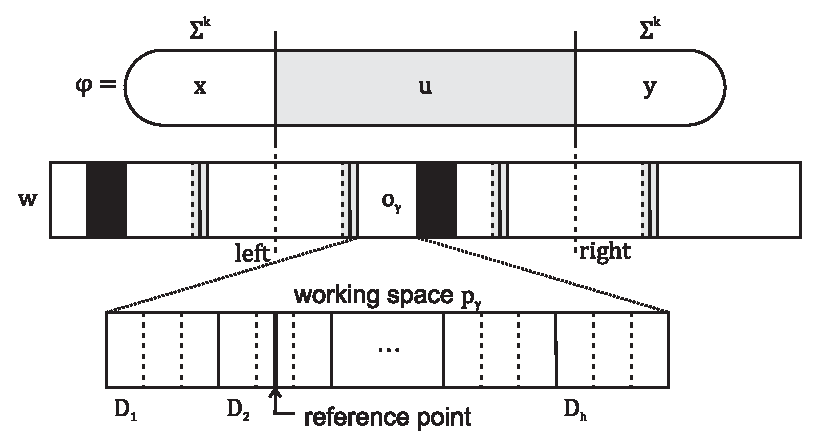
\includegraphics[scale=1.0]{img/instruction_and_tape.eps}
\caption[The execution of the instruction $\phi$.]
{The execution of the instruction $\phi$.}
\label{figure:instruction_and_tape}
\end{figure}

Algorithm \ref{algorithm:dxclra_instruction} describes the execution of the instruction $\phi$ in detail. The used variables and constants will be defined later. The interpretation of the working space $p_{\gamma}$ is illustrated in Figure \ref{figure:working_space_detail}.

\begin{figure}[htp]
\centering
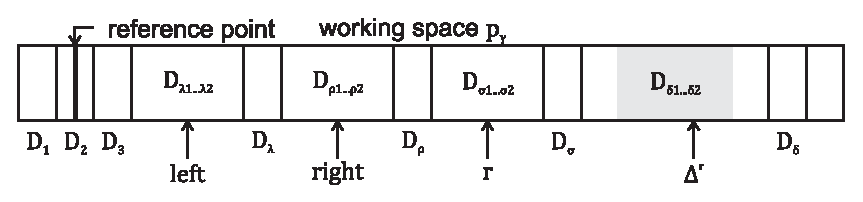
\includegraphics[scale=1.0]{img/working_space_detail.eps}
\caption[The interpretation of the working space $p_{\gamma}$.]
{The interpretation of the working space $p_{\gamma}$.}
\label{figure:working_space_detail}
\end{figure}

\begin{algorithm}
\SetKwInOut{Input}{Input}\SetKwInOut{Output}{Output}
\caption{Executing one step of the instruction $\phi$.}
\label{algorithm:dxclra_instruction}
\DontPrintSemicolon
\LinesNumbered
\Input{Word $w \in \{\lambda, \cent\} \cdot \Gamma^* \cdot \{\lambda, \$\}$, working area $o_{\gamma}$, [instruction $\phi$].}
\nonl From the following steps execute the first step, which has not been executed yet and $\textbf{Halt}$. If you encounter a conflicting step, i.\,e.\ a step which is either not possible to execute or which does not correspond to the information encoded in the working area $o_{\gamma}$, then $\textbf{Reject}$.\;
Mark the unit $D_2$. The corresponding $\Delta$ is called the {\em reference point}.\label{algorithm:dxclra_instruction_step_1}\;
\nonl Let $\textsf{left}$ be the position of the first letter of $u$ relative to the reference point, $\textsf{right}$ be the position of the last letter of $u$ relative to the reference point. Compute $j$ and $s = m_0 + m_2 (i - 1) + (j - 1)$. If the instruction $\phi$ is not provided at the input, compute these values from the information encoded in the corresponding units. If it is not possible, i.\,e.\ the units $D_{\lambda}$, $D_{\rho}$, $D_{\sigma}$, $D_{\delta}$ have not been marked yet, $\textbf{Reject}$.\;
Encode $\textsf{left}$ into the units $D_{\lambda_1}, \ldots, D_{\lambda_2}$. Mark the unit $D_{\lambda}$.\label{algorithm:dxclra_instruction_step_2}\;
Encode $\textsf{right}$ into the units $D_{\rho_1}, \ldots, D_{\rho_2}$. Mark the unit  $D_{\rho}$.\label{algorithm:dxclra_instruction_step_3}\;
Encode $s$ into the units $D_{\sigma_1}, \ldots, D_{\sigma_2}$. Mark the unit $D_{\sigma}$.\label{algorithm:dxclra_instruction_step_4}\;
Mark the unit $D_{\delta}$.\label{algorithm:dxclra_instruction_step_5}\;
Encode the segment $\Delta^r$ (with holes) into the units $D_{\delta_1}, \ldots, D_{\delta_2}$.\label{algorithm:dxclra_instruction_step_6}\;
Clear all letters from the end of the segment $\Delta^r$ (with holes) to the position $\textsf{right}$.\label{algorithm:dxclra_instruction_step_7}\;
Clear all letters from the position $\textsf{left}$ to the beginning of the segment $\Delta^r$ (with holes).\label{algorithm:dxclra_instruction_step_8}\;
\end{algorithm}

Algorithm \ref{algorithm:dxclra_instruction} is designed in such a way, that at any time it is possible to determine unambiguously which steps have already been executed and which are still pending. Every step of the algorithm is consistent with some instruction $\phi$ of the automaton $M$,  therefore, the solver cannot accept more than $M$. We will show later that it is possible to define the parameters and constants used in the solver in such a way, that every instruction of $M$ can be simulated by the solver. Moreover, by using the length-reducing version of coding it is possible to obtain a length-reducing version of the solver, which shortens the word in every step.

The reference point not only reserves the working area $o_{\gamma}$ (the units $D_1$ and $D_3$ must remain empty), but it also exactly defines the relative positions of the first and the last letter of the word $u$. The number $\textsf{left}$ is defined as the number of letters of the shortest prefix of $u$ containing the reference point. By analogy, the number $\textsf{right}$ is defined as the number of letters of the shortest suffix of $u$ containing the reference point.

Steps \ref{algorithm:dxclra_instruction_step_1} to \ref{algorithm:dxclra_instruction_step_5} are nondestructive, i.\,e.\ we are able to recover all symbols $\Delta$ created by these steps. However, when we start creating the continuous segment $\Delta^r$ (with holes) we lose the ability to recover all symbols $\Delta$ in the working area $o_{\gamma}$. Therefore, as we start creating this segment, the information specifying how to complete the execution of the instruction $\phi$ must already be completely encoded in the working area $o_{\gamma}$. We use the standard binary representation for numbers and we always encode the bits from the least significant bit to the most significant bit in a direction from left to right. For all numbers $\textsf{left}$, $\textsf{right}$, and $r$ we use a fixed number of bits. Therefore, it is easy to recognize the markings in the units $D_{\lambda}$, $D_{\rho}$, $D_{\sigma}$ and $D_{\delta}$.

If the unit $D_{\delta}$ is marked then we are in the phase of creating the segment $\Delta^r$ (with holes), i.\,e.\ Step \ref{algorithm:dxclra_instruction_step_6}. We build this segment step by step from left to right by replacing the letters in the subword $D_{\delta_1}, \ldots, D_{\delta_2}$ by the symbol $\Delta$. After completing this segment we move to the next Step \ref{algorithm:dxclra_instruction_step_7}. Note that before we execute Step \ref{algorithm:dxclra_instruction_step_7} the newly created segment $\Delta^r$ (with holes) is not a valid fixed point, since this segment is placed between two marked units (the reference point and the marked unit  $D_{\delta}$). After executing Step \ref{algorithm:dxclra_instruction_step_7} this segment becomes a valid fixed point. This is because we clear the marked unit $D_{\delta}$ and all the areas neighboring with the working area $o_{\gamma}$ are empty (if they exist). Therefore, we need to choose the parameter $j$ in such a way, that the newly defined groups of length $B$, defined by the newly created fixed point of the type $\Delta^r$ (with holes), are exactly the same groups as the original groups before executing Step \ref{algorithm:dxclra_instruction_step_7}. In Step \ref{algorithm:dxclra_instruction_step_8} this problem does not arise, because the groups of length $B$  are always defined relatively to the right of a fixed point.

We conclude this section by mentioning one specific problem concerning Step \ref{algorithm:dxclra_instruction_step_7} and Step \ref{algorithm:dxclra_instruction_step_8}. The problem is, that the position $\textsf{left}$ ($\textsf{right}$, respectively) can cross the fixed point of the type $\mathbf{u} \Delta \mathbf{v} \Delta$ (see Figure \ref{figure:delete_issue}).

\begin{figure}[htp]
\centering
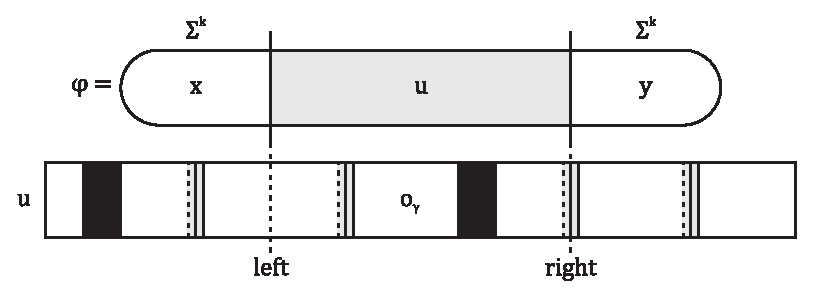
\includegraphics[scale=1.0]{img/delete_issue.eps}
\caption[Problem with the fixed point of the type $\mathbf{u} \Delta \mathbf{v} \Delta$.]
{Problem with the fixed point of the type $\mathbf{u} \Delta \mathbf{v} \Delta$.}
\label{figure:delete_issue}
\end{figure}

The positions $\textsf{left}$ and $\textsf{right}$ are fixed and we cannot change them (these positions are defined by the instruction $\phi$). Fortunately, it does not matter if we damage the fixed point of the type $\mathbf{u} \Delta \mathbf{v} \Delta$. This is because the newly created fixed point of the type $\Delta^r$ (with holes) defines the groups of length $B$ in exactly the same way as did the damaged fixed point. Moreover, thanks to the holes in the newly created fixed point we do not lose even the ability to exactly define the borders of this newly created fixed point. The only issue is that we lose the ability to recover the $\Delta$ symbol(s) of the damaged fixed point. Fortunately, these $\Delta$ symbols are close enough to the newly created segment $\Delta^r$ (with holes), so they are part of the separator corresponding to this segment. As we have already mentioned, the letters in the separator can be set arbitrarily. Therefore, if we want to recover these symbols $\Delta$ corresponding to the damaged fixed point, we can use any letter we want.

Note that the position $\textsf{left}$ ($\textsf{right}$, respectively) cannot cross the fixed point of the type $\Delta^r$ (with holes), because  the word $xuy$ covers always the whole code of the nonterminal  (including its separators).

\subsection{Choosing the Parameters}\label{section:dxclra_parameters}

In this section we define all the parameters and constants used in the previous sections. Let $\Sigma$ be a given alphabet and $G$ be a context-free grammar with $m$ nonterminals.

First we set $m_0 := 8$. Thanks to this setting, each segment $\Delta^r$ (with holes) will contain $\Delta^4$ as a subword. This is how we recognize such segments.

Each group is $B = |\Sigma|$ letters long (since we use Coding 1) and each unit is (by definition) $3 B$ letters long. The parameter $m_2$ defines the range for the parameter $j$ in Algorithm \ref{algorithm:dxclra_instruction}. Since we need this parameter $j$ only to correctly adjust the groups of length $B$ defined by the newly created fixed point, it suffices to choose $m_2 = 3 B$.

The following computations will involve the parameter $h$, which represents the number of units necessary to allow the execution of Algorithm \ref{algorithm:dxclra_instruction}.

The numbers $\textsf{left}$ and $\textsf{right}$ are bounded above by the width of the instruction $\phi$, i.\,e.\ by the constant $2c$, where $c = U + m_1 - 1$ and $U = m_0 + m_2 m - 1 + 2k$. Therefore, to encode such a number we need at most $\lceil \log_2(2c) \rceil$ units. The number $r$ is bounded above by $m_0 + m_2 m$. Observe that this upper bound depends neither on $m_1$, nor on $k$. To encode $r$ we need at most $\lceil \log_2(m_0 + m_2 m) \rceil$ units. Finally, to create the segment $\Delta^r$ (with holes) we need at most $r$ letters, i.\,e.\ at most $\lceil \frac{m_0 + m_2 m}{3 B} \rceil$ units. Therefore, we need at most
$$h = O(m_0 + m_2 m + \log(m_1 + 2k)).$$

By Lemma \ref{lemma:dxclra_t} $m_1, k = \Theta(t)$. Therefore, for any real $\alpha > 0$, there exists a big enough $t$ such that $\alpha t$ is bigger than $h$. By using this technique we can guarantee, for any instruction $\phi = (x, u \to \Delta^r, y)$, a big enough subword $v \in \Sigma^{\ge t}$ of the word $u$. This subword $v$ will guarantee us the existence of a long enough working area $o_{\gamma}$ inside this subword $v$. In our case it is not sufficient only to say that $v \in \Sigma^{\ge t}$ is long enough, because in our algorithm this subword can be interrupted by fixed points of the type $\mathbf{u} \Delta \mathbf{v} \Delta$. The fact that $v \in \Sigma^*$ only means that we are able to recover the symbols $\Delta$ of these fixed points. However, if $v$ is long enough then there will be many of these fixed points and therefore also many of the corresponding working areas. Therefore, it will always be possible to choose one such area $o_{\gamma}$ with empty neighbors.

Let us set $\alpha = \frac{1}{6} \frac{1}{3 B}$, and let $t$ be the smallest positive integer such that for the corresponding parameters $m_1$ and $k$ the following holds:
$$\frac{1}{6} \frac{1}{3 B} t > h.$$
In the first phase of our algorithm let us distribute the fixed point throughout the input working tape in such a way that the corresponding working spaces between any two consecutive fixed points contain at least $2h$ units. Since $t$ is bigger than the length of $6 h$ units, it is easy to see that we will always be able to find a long enough working area $o_{\gamma}$ inside the subword $v \in \Sigma^{\ge t}$.

Also note that during the course of our algorithm the length of every working area will be bounded from above by $2h$ units. This is because the fact that during the course of our algorithm we only replace some segments by new fixed points, so it is not possible to enlarge any working area in this way.

Finally, the constant $K$ of the querier must be long enough to enable us to see any instruction $\phi$ of $M$ as a whole, plus some extra working spaces on both sides of this instruction. It is sufficient to set $K = O(c + h) = O(c)$.

\subsection{Length-Reducing Algorithm}\label{section:dxclra_length-reducing}

In is not difficult to modify Algorithms \ref{algorithm:dxclra_solver} and \ref{algorithm:dxclra_instruction} in order to work with the length-reducing version of Coding 1 (see Section \ref{section:dxclra_coding}). We only need to redefine the length of the word $| \cdot |$ to a weighted sum of its letters, where the letters from $\Sigma$ have the weight $1$ and the symbol $\Delta$ has the weight equal to $\kappa + 1$, where $\kappa$ is the reduction factor from $\kappa$-Reducing Coding 1 Theorem \ref{theorem:dxclra_k_reducing_coding_1}. Moreover, in order to create the segment $\Delta^r$ (with holes) we need now $(\kappa + 1)$ times more letters, i.\,e.\ (at most) $(\kappa + 1) (m_0 + m_2 m)$ letters. When we create the segment $\Delta^r$ (with holes) we always rewrite $\kappa + 1$ consecutive letters from $\Sigma$ to one symbol $\Delta$. It is easy to see that the constant $\kappa$ can be easily incorporated into the previous consideration in Section \ref{section:dxclra_parameters}.

\section{Limited Context Restarting Automata}\label{section:lcra}

The main source for this section is \cite{OCM13}, although here we use a sligthly different notation that is compatible with the rest of this thesis.

In \cite{B11} \emph{limited context restarting automata} were defined as an extension of clearing restarting automata. Also these automata apply rewrite steps only based on context information, but their rewrite rules are more general. In fact, the most general form of these automata accepts exactly the growing context-sensitive languages. In addition, in~\cite{B11} a special version of a genetic algorithm is proposed to learn these automata from positive and negative samples. Here we introduce a slightly generalized version which uses weight-reducing rules instead of length-reducing ones.

In Sections \ref{section:ordinary_lcra} and \ref{section:confluent_lcra} we study the correspondence between limited context restarting automata and McNaughton families of languages of~\cite{Beaudry2003}, among which the class \GCSL\ of \emph{growing context-sensitive languages} \cite{Buntrock19981,DW86}, the class \CRL\ of \emph{Church-Rosser languages}~\cite{MNO88}, and the class {\sf con-gen-mon-McNL} of \emph{confluent generalized monadic McNaughton languages}~\cite{Leupold2011} will appear prominently.

\begin{definition}\label{DefLCRA}[\cite{OCM13}]
A {\em limited context restarting automaton} $M$ ($\lcRA$ $M$, for short) is simply a weight-reducing context rewriting system $M=(\Sigma,\Gamma,\Phi)$ (see Definitions \ref{definition:crs} and \ref{definition:crs-types}).
\end{definition}

\begin{example}
Let $M=(\{a,b,c\},\{a,b,c\},\Phi)$ be the $\lcRA$ that is defined by the set of instruction $\Phi=\{\rarule{\lambda}{\underline{acbb}}{c}{\lambda},\rarule{\cent}{\underline{c}}{\lambda}{\$}\}$. Then $aa\underline{acbb}bbbb \vdash_M a\underline{acbb}bb \vdash_M \underline{acbb} \vdash_M \underline{c} \vdash_M \lambda$, and so the word $a^3cb^6$ belongs to $L(M)$. It is easily seen that $L(M) = \{\, a^ncb^{2n} \mid n \ge 0 \,\}$.
\end{example}

Recall from Definition~\ref{DefLCRA} that all instructions of an $\lcRA$ are necessarily weight-reducing. These most general $\lcRA$ are said to be of type~$\mathcal{R}_0'$. We now define some restricted types of $\lcRA$ by putting additional restrictions on the form of their instructions. We say that an $\lcRA$ $M=(\Sigma,\Gamma,\Phi)$ is of type

\begin{itemize}
\item[$\bullet\;\mathcal{R}_1'$,] if for every $\rarule{u}{x}{y}{v} \in \Phi$: $|y|\le 1$, and $x \in \Gamma^+$;
\item[$\bullet\;\mathcal{R}_2'$,] if for every $\rarule{u}{x}{y}{v} \in \Phi$: $|y|\le 1$, $u \in \{\lambda,\leftsentinel\}$, $v \in \{\lambda,\rightsentinel\}$, and $x \in \Gamma^+$;
\item[$\bullet\;\mathcal{R}_3'$,]  if $\Phi$ only contains instructions of the form $\rarule{u}{x}{y}{\rightsentinel}$, where $|y|\le 1$, $u \in \{\lambda,\leftsentinel\}$, and $x \in \Gamma^+$;
\end{itemize}

We say that an $\lcRA$ $M=(\Sigma,\Gamma,\Phi)$ is of type $\mathcal{R}_i$, for $i \in \{0, 1, 2, 3\}$, if $M$ is of type $\mathcal{R}_i'$ and $\Phi$ only contains length-reducing instructions.

\subsection{Restricted Types}\label{section:ordinary_lcra}

For any $\mathcal{R} \in \{\mathcal{R}_0,\mathcal{R}_0',\mathcal{R}_1,\mathcal{R}_1',\mathcal{R}_2,\mathcal{R}_2',\mathcal{R}_3,\mathcal{R}_3'\}$, we will refer to $\lcRA$ of type $\mathcal{R}$ as ${\lcRA}[\mathcal{R}]$. In~\cite{B10Diploma}, Basovn{\'\i}k  studied length-reducing $\lcRA$, obtaining the following three characterizations.

\begin{theorem}{\rm \cite{B10Diploma}}\label{ThmBasovnik} \\[+0.2cm]
${\rm (a)}\;  {\mathcal L}(\lcRA[0]) = \GCSL.\;
{\rm (b)}\; {\mathcal L}(\lcRA[2]) = \CFL.\;
{\rm (c)}\; {\mathcal L}(\lcRA[3]) = \Reg.$
\end{theorem}

In the current section we complete these results by also studying the other five types of $\lcRA$.
\vspace{+0.2cm}

Let $M = (\Sigma,\Gamma,\Phi)$ be an $\lcRA$. With $M$ we can associate the finite string-rewriting system $R(M) = \{\,uxv\to uyv\mid \rarule{u}{x}{y}{v}\in \Phi\,\}.$ Then $R(M)$ induces a \emph{reduction relation} $\Rightarrow_{R(M)}^*$ on the set of bordered words $\cent\cdot\Gamma^*\cdot\$$, which is the reflexive and transitive closure of the \emph{single-step reduction relation} $\Rightarrow_{R(M)}$ 
that is defined as follows:
$$\begin{array}{c}
\cent w\$\Rightarrow_{R(M)}\cent z\$
\text{ iff }\\
\exists \alpha,\beta\in(\Gamma\cup\{\cent,\$\})^*\,\exists (\ell\to r)\in R(M):
   \cent w\$ = \alpha \ell\beta \textup{ and } \cent z\$ = \alpha r\beta.
\end{array}$$
Thus, for all $w,z\in\Gamma^*$, we have $\cent w\$ \Rightarrow_{R(M)}\cent z\$$ iff $w \vdash_M z$ holds. Accordingly, we see that
$$L(M) = \{\,w\in\Sigma^*\mid w\vdash_M^*\lambda\,\}
       = \{\,w\in\Sigma^*\mid \cent w\$\Rightarrow_{R(M)}^*\cent \$\,\}.$$
By taking $S(M) = R(M) \cup \{\cent \$\to Y\}$, where $Y$ is a new letter, we obtain a finite string-rewriting system on $\Gamma'=\Gamma\cup\{\cent,\$,Y\}$ such that $L(M) = \{\,w\in\Sigma^*\mid \cent w\$ \Rightarrow_{S(M)}^*Y\,\}$ holds. It follows that $L(M)$ is the \emph{McNaughton language} that is specified by the four-tuple $(S(M),\cent,\$,Y)$.
\vspace{+0.2cm}

If $M$ is of type $\mathcal{R}_0'$, then the string-rewriting system $S(M)$ is weight-reducing. Hence, it follows from Theorem~\ref{ThmMcNL}(a) that $L(M)\in\GCSL$. In fact, we will establish the following characterization, extending Theorem~\ref{ThmBasovnik}(a).

\begin{theorem}\label{PropR0}
${\mathcal L}(\lcRAp[0]) = {\mathcal L}(\lcRA[0]) =  \GCSL.$
\end{theorem}

\noindent
\begin{proof}
Because of the above observation, it suffices to show that each growing context-sensitive language is accepted by some $\lcRA$ of type~$\mathcal{R}_0$. Hence, assume that $L\subseteq\Sigma^*$ is growing context-sensitive. We construct an $\lcRA[0]$ $M$ for~$L$. As $L$ is growing context-sensitive, there exists a length-reducing two-pushdown automaton (\TPDA, for short, see, e.\,g.,~\cite{Buntrock19981}) $T = (Q,\Sigma,\Gamma,\delta,$ $q_0,\bot,\lambda,\lambda,\{q_f\})$ that accepts~$L$. Here $\Gamma$ is the tape alphabet of $T$ that includes the input alphabet $\Sigma$ as well as the special bottom marker~$\bot$ for the pushdowns. Thus, for all $w\in\Sigma^*$, $w\in L$ if and only if $T$ accepts starting from the initial configuration $\bot q_0w\bot$, that is, if and only if $\bot q_0 w\bot\vdash_T^* q_f$ holds (see \cite{N2005} Lemma 3.4 and Lemma 4.1). Actually, we may even assume without loss of generality that the initial step of a computation of $T$ that starts from an initial configuration of the form $\bot q_0w\bot$ reduces the overall length of the configuration by at least two, and that $T$ never enters its initial state $q_0$ during a computation.

Let $\overline{\Gamma}=\{\,\overline{a} \mid a\in  \Gamma\,\}$ be a new alphabet in one-to-one correspondence to $\Gamma$ such that $Q$, $\Gamma$, and $\overline{\Gamma}$ are pairwise disjoint, let $\overline{\phantom{a}}:\Gamma^*\to {\overline{\Gamma}}^*$ denote the corresponding isomorphism that is induced by $a\mapsto\overline{a}$ ($a\in\Gamma$), and let $\Delta = Q\cup\Gamma \cup \overline{\Gamma}$. In analogy to the proof of \cite{N2005} Lemma 4.1, we can construct a finite length-reducing string-rewriting system $R$ on $\Delta$ such that, for all $w\in\Sigma^*$, $w\in L \textup{ iff }  \overline{\bot}q_0w\bot \Rightarrow_R^*q_f.$ Here the final state $q_f$ is introduced by specific rules of the form $\overline{\bot} \overline{u} qv\bot \to q_f$. Now from~$R$ we obtain an $\lcRA$ $M = (\Sigma,\Delta,\Phi)$ by taking
$$\begin{array}{lcl}
\Phi  & = &\{\,(\lambda, \ell\to r, \lambda)\mid (\ell\to r)\in R,|\ell|_{\overline{\bot}}=|\ell|_\bot=0\,\}\;\cup\\
      &   &\{\,(\cent, u\to v, \lambda)\mid (\overline{\bot}u\to \overline{\bot}v)\in R, |u|_\bot = 0 =|u|_{q_0}\, \}\;\cup\\
%\end{array}$$
%$$\begin{array}{lcl}   
   &   &\{\,(\cent, u\to v, \lambda)\mid (\overline{\bot}q_0u\to \overline{\bot}v)\in R, |u|_\bot = 0\, \}\;\cup\\
   &   &\{\,(\lambda, u\to v, \$)\mid (u\bot\to v\bot)\in R, |u|_{\overline{\bot}} = 0\, \}\;\cup\\
%\end{array}$$
%$$\begin{array}{lcl}   
   &   &\{\,(\cent, u\to v, \$)\mid (\overline{\bot}u\bot\to \overline{\bot}v\bot)\in R, |u|_{q_0}=0\, \}\;\cup\\
   &   &\{\,(\cent, u\to v, \$)\mid (\overline{\bot}q_0u\bot\to \overline{\bot}v\bot)\in R\, \}\;\cup\\
%\end{array}$$
%$$\begin{array}{lcl}  
   &   &\{\,(\cent, u\to \lambda, \$)\mid (\overline{\bot}q_0u\bot\to q_f)\in R,|u|>0 \}\;\cup\\
   &   &\{\,(\cent, u\to\lambda,\$) \mid (\overline{\bot}u\bot\to q_f)\in R, |u|_{q_0}=0\,\}.\\
\end{array}$$
Then $M$ is of type $\mathcal{R}_0$, and for all $w\in\Sigma^+$,
$$w\in L(M) \;\Leftrightarrow\;  w\vdash_M^*\lambda
            \;\Leftrightarrow\;  \cent w\$ \Rightarrow_{R(M)}^* \cent \$
            \;\Leftrightarrow\;  \overline{\bot}q_0 w\bot \Rightarrow_R^* q_f
            \;\Leftrightarrow\;  w\in L.$$
Thus, $L(M)\, \dot{=}\, L$. This completes the proof of Theorem~\ref{PropR0}.
\end{proof}

Let $G=(N,T,S,P)$ be a weight-increasing context-sensitive grammar, that is, there exists a weight function $g$ such that $g(\ell) < g(r)$ for each rule $(\ell\to r)$ of $P$, and in addition, each rule $(\ell\to r)$ has the form $\ell=uAv$ and $r=uxv$ for some $A\in N$, $u,v\in(N\cup T)^*$, and $x\in (N\cup T)^+$. By taking
$$\Phi(G)  =  \{\,\rarule{u}{x}{A}{v} \mid (uAv\to uxv)\in P\,\}\; \cup
              \{\,\rarule{\cent}{r}{\lambda}{\$} \mid (S\to r)\in P\,\},$$
we obtain an $\lcRA$ $M(G) = (T,N\cup T,\Phi(G))$. It is easily seen that $M(G)$ is of type $\mathcal{R}_1'$, and that $L(M(G))$ $ = L(G)\cup\{\lambda\}$ holds. Thus, ignoring the special case of the empty word we see that all languages that are generated by weight-increasing context-sensitive languages are accepted by \lcRAp[1]. However, the class of languages that are generated by weight-increasing context-sensitive grammars, which is known as the class $\ACSL$ of \emph{acyclic context-sensitive languages}, coincides with the class \GCSL\ of growing context-sensitive languages~\cite{NiWo01}. Hence, we obtain the following characterization.

\begin{theorem}\label{PropR1a}
${\mathcal L}(\lcRAp[1]) =  \GCSL.$
\end{theorem}

If $M = (\Sigma,\Gamma,\Phi)$ is an $\lcRA[1]$, then the rules of $R(M)$ have the form $(uxv \to uyv)$, where $|x|>|y|$ and $|y|\le 1$. By replacing each instruction of the form $\rarule{u}{x}{\lambda}{v}\in \Phi$ by finitely many rules with a revised context, the following technical result can be derived.

\begin{lemma}\label{LemR1a}
If $M = (\Sigma,\Gamma,\Phi)$ is an $\lcRA[1]$, then there exists an equivalent $\lcRA$ $M'=(\Sigma,\Gamma,\Phi')$ of type $\mathcal{R}_1$ such that $|y|=1$ for all instructions $\rarule{u}{x}{y}{v}\in \Phi'$ satisfying $u\not=\cent$ or $v\not=\$$. In fact, for all $w,z\in \Gamma^*$, $w\vdash_M z$ if and only if $w\vdash_{M'} z$.
\end{lemma}

\begin{proof}
To obtain $M'$ from $M$, we simply replace each instruction of the form $\phi=\rarule{u}{x}{\lambda}{v}\in \Phi$. If $u=u_1A$ for some $A\in\Gamma$, then we replace $\phi$ by the instruction $\phi'=\rarule{u_1}{Ax}{A}{v}$; if $u=\lambda$ or $u=\cent$ and $v=Bv_1$ for some $B\in\Gamma$, then we replace $\phi$ by the instruction $\phi'=\rarule{u}{xB}{B}{v_1}$; if $u =\cent$ and $v=\lambda$, then we replace $\phi$ by the set of instructions $\Phi'(\phi) = \{\,\rarule{\cent}{xA}{A}{\lambda}\mid A\in \Gamma\,\} \,\cup\,\{\rarule{\cent}{x}{\lambda}{\$}\}$; if $u=\lambda$ and $v=\$$, then we replace $\phi$ by the set of instructions $\Phi'(\phi) = \{\,\rarule{\lambda}{Ax}{A}{\$}\mid A\in \Gamma\,\} \,\cup\,\{\rarule{\cent}{x}{\lambda}{\$}\}$; and if $u=\lambda=v$, then we replace $\phi$ by the set of instructions $\Phi'(\phi) = \{\,\rarule{\lambda}{xA}{A}{\lambda},\rarule{\lambda}{Ax}{A}{\lambda}\mid A\in \Gamma\,\} \,\cup\,\{\rarule{\cent}{x}{\lambda}{\$}\}$. Then, for all $w,z\in\Gamma^*$, if $w\vdash_M z$ using instruction~$\phi$, then $w\vdash_{M'} z$ by instruction $\phi'$ or by one of the instructions of $\Phi'(\phi)$, and conversely, if $w\vdash_{M'} z$ by instruction $\phi'$ or by one of the instructions of $\Phi'(\phi)$, then $w\vdash_M z$ by instruction~$\phi$.
\end{proof}

Let $M=(\Sigma,\Gamma,\Phi)$ be an $\lcRA[1]$ that satisfies the properties of Lemma~\ref{LemR1a}, let $R(M)$ be the corresponding string-rewriting system, and let $R(M)^{-1}$ denote the system $R(M)^{-1} = \{\,(v\to u) \mid (u\to v)\in R(M)\,\}.$ From $R(M)^{-1}$ we can construct a length-increasing context-sensitive grammar $G(M) = (\Gamma',\Sigma',S,R')$ that generates the language $L(G(M)) = \cent\cdot L(M)\cdot\$$. Thus, the language $\cent\cdot L(M)\cdot\$$ is a growing acyclic context-sensitive language  (see, e.\,g.,~\cite{NiWo01}). It is known from~\cite{BunHabil} that the class $\GACSL$ of \emph{growing acyclic context-sensitive languages} is closed under the operations of removing left and right end markers. Hence, the language $L(M)$ is growing acyclic context-sensitive, too. Conversely, if $G=(N,T,S,P)$ is a length-increasing context-sensitive grammar, then by taking
$$
\Phi(G)  =  \{\,\rarule{u}{x}{A}{v} \mid (uAv\to uxv)\in P\,\}\; \cup
            \{\,\rarule{\cent}{r}{\lambda}{\$}\mid (S\to r)\in P\,\},
$$
we obtain an $\lcRA$ $M(G) = (T,N\cup T,\Phi(G))$ of type $\mathcal{R}_1$ such that $L(M(G)) = L(G)\cup\{\lambda\}$ holds. Thus,  we have the following characterization.

\begin{theorem}\label{PropR1b}
${\mathcal L}(\lcRA[1]) = \GACSL.$
\end{theorem}

It is known that the class $\GACSL$ properly contains the class $\CFL$ of context-free languages, and it is obviously contained in $\ACSL = \GCSL$. However, it is an open problem whether this containment is strict or not.
\vspace{+0.1cm}

Let $M = (\Sigma,\Gamma,\Phi)$ be an \lcRA[2']. Then, for each instruction $\rarule{u}{x}{y}{v}\in \Phi$, we have $u\in\{\lambda,\cent\}$, $v\in\{\lambda,\$\}$, $|x|\ge 1$, $|y|\le 1$, and $g(x)>g(y)$ for a fixed weight function~$g$. Hence, the corresponding string-rewriting system $R(M)$ can be split into four disjoint subsystems:
$$\begin{array}{llcll}
{\rm (a)} & R_{bif} & = & \{\,\cent x\$ \to \cent y\$ \mid \rarule{\cent}{x}{y}{\$}\in \Phi\,\}, & \textup{the \emph{bifix rules} of }R(M),\\
{\rm (b)} & R_{pre}& = & \{\,\cent x \to \cent y \mid \rarule{\cent}{x}{y}{\lambda}\in \Phi\,\}, & \textup{the \emph{prefix rules} of }R(M),\\
{\rm (c)} & R_{suf}& = & \{\,x\$ \to y\$ \mid \rarule{\lambda}{x}{y}{\$}\in \Phi\,\}, & \textup{the \emph{suffix rules} of }R(M),\\
{\rm (d)} & R_{inf}& = & \{\,x \to y \mid \rarule{\lambda}{x}{y}{\lambda}\in \Phi\,\}, & \textup{the \emph{infix rules} of }R(M).\\
\end{array}$$
Let $B(M) = \{\,\alpha\in\Gamma^*\mid \cent \alpha\$\in {\rm dom}(R_{bif}) \textup{ and }
\cent \alpha\$\Rightarrow_{R(M)}^* \cent \$\,\}\,\cup\,\{\lambda\}.$ As $R(M)$ is finite, so is the set~$B(M)$. Let $R' = R_{pre}\cup R_{suf}\cup R_{inf}$. Then
$$
L(M)  =   \{\,w\in\Sigma^*\mid \cent w\$\Rightarrow_{R(M)}^*\cent\$\,\}
      =   \{\,w\in\Sigma^*\mid \exists \alpha\in B(M):\cent w\$\Rightarrow_{R'}^*\cent \alpha\$\,\},
$$
that is, $\cent\cdot L(M) \cdot \$ = \nabla_{R'}^*(\cent\cdot B(M)\cdot\$) \cap (\cent\cdot\Sigma^*\cdot\$),$ where $\nabla_{R'}^*(\alpha)$ denotes the \emph{set of ancestors} of $\alpha$ mod~$R'$, and $\nabla_{R'}^*(B) = \bigcup_{\alpha\in B}\nabla_{R'}^*(\alpha)$ for any set~$B$. Now we define a mixed rewriting system (see, e.\,g.,~\cite{Hofbauer2004301}) $P(M)=P_{pre}\cup P_{suf}\cup P_{inf}$ by taking the {\em prefix-rewriting system}\footnote{The rules of a prefix-rewriting system can only be applied to the prefix of a word.} $P_{pre}  =  \{\,x \to  y \mid (\cent x\to \cent y)\in R_{pre}\,\}$, the {\em suffix-rewriting system}\footnote{The rules of a suffix-rewriting system can only be applied to the suffix of a word.} $ P_{suf}  =  \{\,x \to  y \mid (x\$\to y\$)\in R_{suf}\,\}$, and the {\em string-rewriting system}  $P_{inf}  =  R_{inf}$. Then $L(M) = \nabla_{P(M)}^*(B(M))\cap\Sigma^*.$ As $P(M)$ only contains \emph{generalized monadic rules} (see, e.\,g.,~\cite{Leupold2011}), it follows that the set $\nabla_{P(M)}^*(B(M))$ is context-free, which in turn implies that $L(M)$ is a context-free language.

Conversely, if $L\subseteq\Sigma^*$ is a context-free language, then there exists a context-free grammar $G=(N,\Sigma,S,P)$ for $L\cap\Sigma^{\ge 2}$ such that, for each rule $(\ell\to r)$ of $P$, we have $|\ell|=1$ and $|r|=2$. We now obtain an $\lcRA$ $M(G)=(\Sigma,N\cup\Sigma,\Phi)$ by taking
$$\Phi = \{\,\rarule{\lambda}{r}{\ell}{\lambda}\mid (\ell\to r)\in P\,\}\,\cup\,
         \{\,\rarule{\cent}{a}{\lambda}{\$}\mid a\in(\Sigma\cap L)\cup\{S\}\,\}.$$
Then $M(G)$ is of type $\mathcal{R}_2$, and $L(M(G))\,\dot{=}\,L$. Thus, we have the following characterization.
\begin{theorem}\label{PropR2}
${\mathcal L}(\lcRAp[2]) = {\mathcal L}(\lcRA[2]) = \CFL.$
\end{theorem}

\begin{figure}
{\small
\[ \xymatrix@R8pt@C5pt{
\txt{${\mathcal L}(\textup{\sf lc-RA}[{\mathcal R}_0])$}\ar@{=}[r] &
\txt{${\mathcal L}(\textup{\sf lc-RA}[{\mathcal R}_0'])$}\ar@{=}[r] & \txt{\sf GCSL} \ar@{=}[r]
                   & \txt{$\textup{\sf lr-McNL}$}\ar@{=}[r] & \txt{$\textup{\sf wr-McNL}$}\\
                                                           &
\txt{${\mathcal L}(\textup{\sf lc-RA}[{\mathcal R}_1'])$}\ar@{=}[u]  \\
                                                           &
\txt{${\mathcal L}(\textup{\sf lc-RA}[{\mathcal R}_1])$} \ar@{->}_?[u]  
                   & \GACSL\ar@{=}[l]\ar@{->}_?[uu]\\
\txt{${\mathcal L}(\textup{\sf lc-RA}[{\mathcal R}_2])$}\ar@{=}[r] &
\txt{${\mathcal L}(\textup{\sf lc-RA}[{\mathcal R}_2'])$}\ar@{=}[r] &
\txt{\sf CFL}\ar@{->}[u]\ar@{=}[r] 
& \txt{$\textup{\sf mon-McNL}$}\ar@{=}[r] & \txt{$\textup{\sf gen-mon-McNL}$}\\
\txt{${\mathcal L}(\textup{\sf lc-RA}[{\mathcal R}_3])$}\ar@{=}[r] &
\txt{${\mathcal L}(\textup{\sf lc-RA}[{\mathcal R}_3'])$}\ar@{=}[r] &
\txt{\sf REG}\ar@{->}[u]\\
}
\]
\caption{Hierarchy of language classes that are accepted by the various types of
limited context restarting automata.
Question marks indicate inclusions not known to be proper.}\label{Fig1}
}
\end{figure}

Finally, let $M = (\Sigma,\Gamma,\Phi)$ be an $\lcRA[3']$, that is, for all instructions $\rarule{u}{x}{y}{v}\in \Phi$, we have $u\in\{\lambda,\cent\}$, $v=\$$, $|x|\ge 1$, $|y|\le 1$, and $g(x)>g(y)$ for a fixed weight function~$g$. Hence, the corresponding string-rewriting system $R(M)$ can be split into two disjoint subsystems:
$$\begin{array}{llcll}
{\rm (a)} & R_{bif} & = & \{\,\cent x\$ \to \cent y\$ \mid \rarule{\cent}{x}{y}{\$}\in \Phi\,\}, & \textup{the \emph{bifix rules} of }R(M),\\
{\rm (b)} & R_{suf}& = & \{\,x\$ \to y\$ \mid \rarule{\lambda}{x}{y}{\$}\in \Phi\,\}, & \textup{the \emph{suffix rules} of }R(M).\\
\end{array}$$
As above, the set $B(M) = \{\,\alpha\in\Gamma^*\mid \cent \alpha\$\in {\rm dom}(R_{bif}) \textup{ and } \cent \alpha\$\Rightarrow_{R(M)}^* \cent \$\,\}\,\cup\,\{\lambda\}$ is finite, and
$$
L(M)  =  \{\,w\in\Sigma^*\mid \cent w\$\Rightarrow_{R(M)}^*\cent\$\,\}
      =  \{\,w\in\Sigma^*\mid \exists \alpha\in B(M):\cent w\$\Rightarrow_{R_{suf}}^* \cent\alpha\$\,\},
$$
that is, $\cent\cdot L(M) \cdot \$ = \nabla_{R_{suf}}^*(\cent\cdot B(M)\cdot\$) \cap (\cent\cdot\Sigma^*\cdot\$).$ For the suffix-rewriting system $P(M) = \{\,y\to x\mid (x\$\to y\$)\in R_{suf}\,\}$, we obtain $L(M) = \Delta_{P(M)}^*(B(M))\cap\Sigma^*.$ As $B(M)$ is finite, and, hence, regular, it follows that the set of descendants $\Delta_{P(M)}^*(B(M))$ of this set with respect to the suffix rewriting system $P(M)$ is regular~\cite{Buc64}, which in turn implies that $L(M)$ is regular.

Conversely, if $L\subseteq\Sigma^*$ is a regular language, then there exists a regular grammar $G=(N,\Sigma,S,P)$ for $L\cap\Sigma^{\ge 2}$ such that, for each rule $(\ell\to r)$ of $P$, we have $\ell\in N$ and $r\in \Sigma\cdot N \cup \Sigma^2$. We now obtain an $\lcRA$ $M(G)=(\Sigma,N\cup\Sigma,\Phi)$ by taking
$$\Phi = \{\,\rarule{\lambda}{r}{\ell}{\$}\mid (\ell\to r)\in P\,\}\,\cup\,
         \{\,\rarule{\cent}{a}{\lambda}{\$}\mid a\in(L\cap\Sigma)\cup\{S\}\,\}.$$
Then $M(G)$ is of type $\mathcal{R}_3$, and $L(M(G))\,\dot{=}\,L$. Thus, we have the following characterization.
\begin{theorem}\label{PropR3}
${\mathcal L}(\lcRAp[3]) = {\mathcal L}(\lcRA[3]) = \Reg.$
\end{theorem}

The results on the various $\lcRA$ are summarized by the diagram in Figure~\ref{Fig1}.

\subsection{Confluent Restricted Types}\label{section:confluent_lcra}

As defined in Definition~\ref{DefLCRA}, an $\lcRA$ $M=(\Sigma,\Gamma,\Phi)$ is a nondeterministic device. A word $w\in\Sigma^*$ belongs to the language $L(M)$ accepted by $M$, if and only if there exists a computation of $M$ that transforms the initial configuration with tape content $\cent w\$$ into the configuration with tape content~$\cent\$$. In general, there will be many different computations of $M$ that start from the configuration with tape content~$\cent w\$$, and only some of them will derive the tape content~$\cent \$$. As this phenomenon complicates the problem of deciding membership in~$L(M)$, we are interested in $\lcRA$ for which all computations from $\cent w\$$ lead to $\cent\$$, if $w\in L(M)$. Actually, as the reduction relation $\vdash_M$ corresponds to the single-step reduction relation $\Rightarrow_{R(M)}$ that is induced by the string-rewriting system $R(M)$ on the set of bordered words $\cent\cdot\Gamma^*\cdot \$$, this would lead to considering $\lcRA$ $M$ for which the string-rewriting system $R(M)$ is \emph{confluent on the congruence class} $[\cent\$]_{R(M)}$. Unfortunately, it is undecidable in general whether a finite string-rewriting system is confluent on a given congruence class, even if the given finite system only contains length-reducing rules~\cite{otto27}. Therefore, we turn to $\lcRA$ that satisfy an even stronger restriction than confluence on a particular congruence class.
%
\begin{definition}\label{DefConf}
An $\lcRA$ $M=(\Sigma,\Gamma,\Phi)$ is called \emph{confluent} if the corresponding string-rewriting system $R(M)$ is confluent.
\end{definition}

As $R(M)$ is a finite and terminating string-rewriting system for each $\lcRA$, confluence is a decidable property of $\lcRA$ (see Proposition~\ref{PropCon} and the subsequent paragraph). We illustrate the above definition by a simple example.

\begin{example}\label{ExConLcR}
 Let $\Sigma=\{a\}$, let $\Gamma = \{a,F\}$, and let 
$\Phi=\{\rarule{\cent}{aaaa}{aaF}{\lambda},$ $\rarule{\lambda}{Faa}{aF}{\lambda},
        \rarule{\lambda}{F}{\lambda}{\$},\rarule{\cent}{aa}{\lambda}{\$},\rarule{\cent}{a}{\lambda}{\$}\}.$ Then $M=(\Sigma,\Gamma,\Phi)$ is an $\lcRA$ of type $\mathcal{R}_0$ that accepts the language $L_{\rm expo}$ (see Example \ref{ExMcNL}), and it is easily checked that $M$ is confluent.
\end{example}

We will use the prefix {\sf con-} to denote types of confluent $\lcRA$. Further, for each type $\mathcal{R}\in\{\,\mathcal{R}_i',\mathcal{R}_i\mid i\in\{0,1,2,3\}\,\}$, {\sf lc-RA$[\textup{\sf con-}\mathcal{R}]$} will denote the class of $\lcRA$ of type $\mathcal{R}$ that are confluent.

In the following we study the expressive power of the various types of confluent $\lcRA$. As in the previous section we consider the various types in turn, from the most general one to the most restricted one.

If $M=(\Sigma,\Gamma,\Phi)$ is an $\conlcRA[0']$, then $S(M) = R(M) \cup  \{\cent\$\to Y\}$ is a finite weight-reducing string-rewriting system that is confluent, and $L(M)$ is simply the McNaughton language that is specified by $(S(M),\cent,\$,Y)$. Thus, $L(M)$ is a \emph{Church-Rosser language}~\cite{MNO88}. On the other hand, if $L\subseteq\Sigma^*$ is a Church-Rosser language, then it is accepted by a length-reducing deterministic two-pushdown automaton~\cite{N2005}. Following the proof of Theorem~\ref{PropR0}, a confluent $\lcRA$ of type $\mathcal{R}_0$ can be constructed for~$L$. Hence, we obtain the following characterization.
%
\begin{theorem}\label{PropConR0}
${\mathcal L}(\conlcRA[0']) = {\mathcal L}(\conlcRA[0]) = \CRL.$
\end{theorem}

In~\cite{Woi03} Woinowski introduced a normal form for presentations of Church-Rosser languages, called \emph{context-splittable Church-Rosser language systems}. Such a presentation is of the form $(S,\cent,\$,Y)$, where $S$ is a finite, weight-reducing, and confluent string-rewriting system that consists of rules of the form $(uxv\to uyv)$, where $u,v\in\Gamma^*$, $x\in\Gamma^+$, and $|y|\le 1$, and rules of the form $(\cent x\$\to Y)$, where $x\in\Gamma^+$. As each Church-Rosser language admits a presentation of this form~\cite{Woi03}, and as a presentation of this form can immediately be translated into an $\lcRA$ of type $\textup{\sf con-}\mathcal{R}_1'$, this gives the following characterization.

\begin{theorem}\label{PropConR1prim}
${\mathcal L}(\conlcRA[1']) = \CRL.$
\end{theorem}

For the class of languages that are accepted by confluent $\lcRA$ of type~$\mathcal{R}_1$,
we have no characterization result yet. On the one hand, these automata can only accept (certain) Church-Rosser languages, and hence, they do not accept all context-free languages. On the other hand, the language  $L_{\rm expo5} = \{\,a^{5^n}\mid n\ge 0\,\}$ is accepted by an $\conlcRA[1]$, as shown in~\cite{OCM12}. As this language is not context-free, we can at least conclude the following.
%
\begin{corollary}\label{CorConR1}
The language class ${\mathcal L}(\conlcRA[1])$ is incomparable to the class $\CFL$ with respect to inclusion.
\end{corollary}

It remains open whether $\lcRA$ of type $\textup{\sf con-}\mathcal{R}_1$ accept all Church-Rosser languages, in fact, it is even open whether they accept at least all deterministic context-free languages.

In the following we present the results concerning the confluent $\lcRA$ of type $\mathcal{R}_2'$ and $\mathcal{R}_2$. We do not give proofs, since these proofs are very complicated and technical. The interested reader is referred to \cite{OCM13}.

\begin{theorem}\label{congenmonMcNL}
$\mathcal{L}(\conlcRA[2']) = \textup{\sf con-gen-mon-McNL}$.
\end{theorem}
%
\begin{theorem}\label{conmonMcNL}
$\mathcal{L}(\conlcRA[2]) \subseteq \textup{\sf con-mon-McNL}$.
\end{theorem}

It currently remains open whether the converse of Theorem~\ref{conmonMcNL} holds.

Finally, we turn to the confluent $\lcRA$ of types  $\mathcal{R}_3'$ and $\mathcal{R}_3$. If $M$ is an $\conlcRA[3']$, then $L(M)$ is a regular language by Theorem~\ref{PropR3}. Conversely, if $L\subseteq\Sigma^*$ is a regular language, then there exists a $\DFA$ $A=(Q,\Sigma,q_0,F,\delta)$ that accepts~$L^R$. We define an $\lcRA$ $M=(\Sigma,Q\cup\Sigma,\Phi)$ as follows, where $a,b\in\Sigma$ and $q,q'\in Q$:
$$\begin{array}{ccl}
\Phi & = & \{\,\rarule{\cent}{ab}{q}{\lambda}  \mid  \delta(q_0,ab)=q\,\}
      \,  \cup \,  \{\,\rarule{\cent}{qa}{q'}{\lambda}  \mid  \delta(q,a)=q'\,\} \,\cup \\
     &   & \{\,\rarule{\cent}{q}{\lambda}{\$}  \mid  q\in F\,\}
      \, \cup  \, \{\,\rarule{\cent}{a}{\lambda}{\$}  \mid a\in \Sigma\cap L^R\,\}.
\end{array}$$
It is easily seen that $L(M)\,\dot{=}\,L^R$, and that the string-rewriting system $R(M)$ is confluent. By taking $M'=(\Sigma,Q\cup\Sigma,\Phi')$, where
$\Phi' = \{\,\rarule{\lambda}{u^R}{v^R}{\$} \mid \rarule{\cent}{u}{v}{\lambda}\in \Phi\,\} 
         \,\cup
         \{\,\rarule{\cent}{u^R}{v^R}{\$} \mid \rarule{\cent}{u}{v}{\$}\in \Phi\,\}$,
we obtain a confluent $\lcRA$ of type $\mathcal{R}_3$ that accepts the language~$L$. Thus, we have the following characterization.
%
\begin{theorem}\label{PropConR3}
${\mathcal L}(\conlcRA[3']) = {\mathcal L}(\conlcRA[3]) = \Reg.$
\end{theorem}

The diagram in Figure~\ref{Fig2} summarizes our results on confluent $\lcRA$.

\begin{figure}
{\small
\[ \xymatrix@R8pt@C15pt{
                              &                      &                   & \txt{\sf GCSL}\\
\txt{${\mathcal L}(\textup{\sf lc-RA}[\textup{\sf con-{$\mathcal R$}}_0])$}\ar@{=}[r] &
\txt{${\mathcal L}(\textup{\sf lc-RA}[\textup{\sf con-{$\mathcal R$}}_0'])$}\ar@{=}[r] &
\txt{\sf CRL}\ar@{->}[ur] & \txt{\sf CFL}\ar@{->}[u]\\
       &  \txt{${\mathcal L}(\textup{\sf lc-RA}[\textup{\sf con-{$\mathcal R$}}_1'])$}\ar@{=}[u] &
\txt{\sf DCFL}\ar@{->}[u]\ar@{->}[ur] \\
     \txt{${\mathcal L}(\textup{\sf lc-RA}[\textup{\sf con-{$\mathcal R$}}_1])$} \ar@{->}_?[ur]  &  &
\txt{\sf symDCFL}\ar@{->}[u]\\
      & \txt{${\mathcal L}(\textup{\sf lc-RA}[\textup{\sf con-{$\mathcal R$}}_2'])$}\ar@{->}[ur]\ar@{->}[uu]
& & \txt{\sf LIN}\ar@{->}[uuu]\\
             & \txt{$\textup{\sf con-gen-mon-McNL}$}\ar@{=}[u]\\
\txt{${\mathcal L}(\textup{\sf lc-RA}[\textup{\sf con-{$\mathcal R$}}_2])$}\ar@{->}_?[r]\ar@{->}[uuu]&
                  \txt{$\textup{\sf con-mon-McNL}$}\ar@{->}_?[u]  \\
\txt{${\mathcal L}(\textup{\sf lc-RA}[\textup{\sf con-{$\mathcal R$}}_3])$}\ar@{=}[r]\ar@{->}[u] &
\txt{${\mathcal L}(\textup{\sf lc-RA}[\textup{\sf con-{$\mathcal R$}}_3'])$}\ar@{=}[r] & \txt{\sf REG}\ar@{->}[uuuu]\ar@{->}[uuur]\\
}
\]
\caption{Hierarchy of language classes that are accepted by the various types of confluent limited context restarting automata. Question marks indicate inclusions not known to be proper.}\label{Fig2}
}
\end{figure}
